\documentclass[runningheads]{llncs}

\usepackage{standalone}
\usepackage{import}
\usepackage{pgfplots}
% \usepackage{color}
\usepackage{tikz}
\usepackage{pgfplots}
\usepgfplotslibrary{fillbetween}
\pgfplotsset{compat=1.16}
\usetikzlibrary {arrows.meta, automata, positioning, fit}
\usepackage{url}
\usepackage{algorithm}
\usepackage{algpseudocode}
\usepackage{amsfonts}
\usepackage{amsmath, amssymb}
\usepackage{float, subcaption, graphics}
\usepackage{mathbbol}
\usepackage{colortbl}
\definecolor{grayshade}{gray}{0.9}
\usepackage{array} % Required for custom column formatting
\usepackage[normalem]{ulem}
% set algorithmicx
\renewcommand{\algorithmicrequire}{\textbf{Input:}}  % Use Input in the format of Algorithm  
\renewcommand{\algorithmicensure}{\textbf{Output:}} % Use Output in the format of Algorithm 

\newcommand*{\Int}{\mathbb{Z}}
\newcommand*{\Nat}{\mathbb{N}}
\newcommand*{\NFA}{\mathcal{A}}
\newcommand{\Lang}{\mathcal{L}}
\newcommand{\cefaout}{\mathcal{O}}
\newcommand*{\op}{o}
\newcommand*{\svars}{{\sf SVars}}
\newcommand*{\ivars}{{\sf IVars}}

\newcommand{\anivar}{\mathfrak{x}}
\newcommand{\anivary}{\mathfrak{y}}
\newcommand{\anivarz}{\mathfrak{z}}

\newtheorem{observation}{Observation}

\newcommand*{\prj}{{\sf prj}}

\newcommand*{\red}[1]{\textcolor{red}{#1}}

\newcommand{\costset}{\mathbb{C}}
\newcommand{\confset}{\mathsf{Conf}}

\newcommand*{\myvec}[1]{\vec{#1}}
\newcommand*{\regex}{e}
\newcommand*{\strsort}{\verb|Str|}
\newcommand*{\intsort}{\verb|Int|}
\newcommand*{\lan}{\mathcal{L}}
\newcommand*{\highlight}[1]{\textbf{\textit{#1}}}
\newcommand*{\aut}{\mathcal{A}}
\newcommand*{\algfun}[1]{\texttt{#1}}
\newcommand*{\strlen}[1]{\texttt{len}(#1)}
\newcommand*{\myemph}[1]{\textcolor{red}{#1}}
\newcommand*{\mult}[1]{$\times$}
\newcommand*{\ostrichrecl}{\rm OSTRICH^{RECL}}
\newcommand*{\emptinessprob}{$SAT_{CEFA}[LIA]$ problem}

\newcommand{\srel}{\mathsf{Rel}}

\newcommand{\ltrue}{\mathtt{true}}
\newcommand{\lfalse}{\mathtt{false}}
%%
\newcommand{\hide}[1]{ }

\newcommand{\cB}{\mathcal{B}}
\newcommand{\cC}{\mathcal{C}}
\newcommand{\cD}{\mathcal{D}}
\newcommand{\cU}{\mathcal{U}}
\newcommand{\fZ}{\mathfrak{Z}}

\newcommand{\concat}{\cdot}

\newcommand{\reclsat}{{\sf SAT_{RECL}}}
\newcommand{\cefadec}{{\sf NE_{LIA}(CEFA)}}

\newcommand{\parikh}{\mathsf{parikh}}

%%%%% comments commands
\newcommand{\zhilin}[1]{\color{orange}\textbf{ZL:} #1 \textbf{:LZ}\color{black}}
\newcommand{\denghang}[1]{{\color{teal}\textbf{DH:} #1 \textbf{:HD}\color{black}}}

%% end of the preamble, start of the body of the document source.
\begin{document}
%%
%% The "title" command has an optional parameter,
%% allowing the author to define a "short title" to be used in page headers.
\title{String Constraints with Regex-Counting and String-Length Solved More Efficiently}

%%
\author{Denghang Hu\inst{1,2} \and
  Zhilin Wu\inst{1,2}\orcidID{0000-0003-0899-628X}}
\authorrunning{Denghang Hu \and Zhilin Wu}
\titlerunning{String Constraints with Counting and Length Solved More Efficiently}
% \authornote{Both authors contributed equally to this research.}

\institute{
State Key Laboratory of Computer Science, \\
Institute of Software, Chinese Academy of Sciences, Beijing, China
\and
University of Chinese Academy of Sciences, Beijing, China \\
\email{\{hudh,wuzl\}@ios.ac.cn}
}


%\institute{State Key Laboratory of Computer Science, \\Institute of Software, Chinese Academy of Sciences\\
%  }

\maketitle

%% The abstract is a summary of the work to be presented in the
%% article.
%\vspace{-6mm}
\begin{abstract}
\subimport{sections/}{abstract.tex}
\end{abstract}

%\zhilin{18 pages, excluding references}\newline
%\denghang{deadline: May 11, 2023 (AoE), 20 hours later than Beijing time (possibly extended:))}

%\vspace{-8mm}
\section{Introduction} \label{sec:intro}
%\vspace{-2mm}
%!TEX root = ../main.tex
%\documentclass[11pt]{standalone}
%\begin{document}

In modern programming languages---such as JavaScript, Python, Java, and PHP---the string data type plays a crucial role. 
It is well-known that string manipulations are error-prone and could even give rise to security vulnerabilities (e.g. \ cross-site scripting, aka XSS). 
One powerful method for identifying such bugs in programs is \emph{symbolic execution} (possibly in combination with dynamic analysis), which analyses symbolic paths in a program by viewing them as constraints, whose feasibility is checked by constraint solvers. 
%
Symbolic execution of string manipulating programs has motivated the highly active research area of \emph{string constraint solving}, resulting in the development of numerous string solvers in the last decade, including the state-of-the-art string constraint solvers, e.g.
Z3seq~\cite{z3seq}, CVC4/5~\cite{cvc4}, Z3str/2/3/4~\cite{Z3-str,Z3-str2,Z3-str3,BerzishMurphy2021}, Z3str3RE~\cite{BD+23}, 
Z3-Trau~\cite{Z3-trau}, OSTRICH~\cite{CHL+19}, Slent~\cite{WC+18}, among many others. 

Regular expressions (abbreviated as regex) and string-length function are widely used in string-manipulating programs. According to the statistics from \cite{CS16,DCSL18,WS18}, regular expressions are used in about 30–40\% Java, JavaScript, and Python software projects. 
Moreover, that string-length function occupies 78\% of the occurrences of string operations in 18 Javascript applications, according to the statistics from \cite{malware_detection_3_kudzu}. 
%Operations like \verb|length| that take string inputs and return an integer frequently appear in real-world JavaScript applications (78\% of string operations in 18 applications)
As a result, most of the aforementioned string constraint solvers support both regular expressions and string-length function. Moreover, specialized algorithms have been proposed to efficiently solve the class of string constraints with regular expressions and string-length function \cite{LTR+15,BD+23}. 
%a decision procedure based on tableaux calculus was designed in \cite{LTR+15} for the class of string constraints with regular expressions and string-length function. The decision procedure has been implemented in CVC4/5 \cite{LRT+16}.

Counting (aka repetition) is a convenient feature in regular expressions that count the number of matchings of sub-patterns. For instance, $a^{\{2, 4\}}$ specifies that $a$ occurs at least twice and at most four times, and $a^{\{2, \infty\}}$ specifies that $a$ occurs at least twice. 
Note that Kleene star and Kleene plus operator can be seen as special cases of counting operator. For instance, $a^*$ and $a^+$ are equivalent to $a^{\{0,\infty\}}$ and $a^{\{1,\infty\}}$.
Counting is a frequently used feature of regular expressions. According to the statistics from \cite{CS16}, Kleene star/plus occur in more than 70\% of 1,204 Python projects, while the other forms of counting occur in more than 20\% of them. Therefore, an efficient analysis of string manipulating programs requires efficient solvers for string constraints that contain at least regular expressions with counting\footnote{In the rest of this paper, for clarity, we use counting to denote expressions of the form $e^{\{m, n\}}$ and  $e^{\{m, \infty\}}$, but not $e^*$ or $e^+$.} and string-length function. 

Nevertheless, the aforementioned state-of-the-art string constraint solvers still suffer from string constraints with regex-counting and string-length, especially when the counting bounds are large. For instance, none of the string solvers CVC5, Z3seq, Z3-Trau, Z3str3, Z3str3RE, and OSTRICH is capable of solving the following constraint within 300 seconds,
%
\begin{equation}\label{eqn-running}
x \in (\Sigma \setminus a)^{\{1, 60\}} (\Sigma \setminus b)^{\{1, 60\}} (\Sigma \setminus c)^{\{0, 60\}} \wedge x \in \Sigma^* c^+ \wedge |x| > 120.
\end{equation}
Intuitively, the constraint in (\ref{eqn-running}) specifies that $x$ is a concatenation of three strings $x_1, x_2, x_3$ where $a$ (resp. $b, c$) does not occur in $x_1$ (resp. $x_2, x_3$), moreover, $x$ ends with a nonempty sequence of $c$'s, and the length of $x$ is greater than $120$. It is easy to observe that this constraint is unsatisfiable since on the one hand, $|x| > 120$ and the counting upper bound $60$ in both $(\Sigma \setminus a)^{\{1, 60\}}$ and $(\Sigma \setminus b)^{\{1, 60\}}$ imply that $x$ must end with some character from $\Sigma \setminus c$, that is, a character different from $c$, and on the other hand, $x \in \Sigma^*c^+$ requires that $x$ has to end with $c$.

A typical way for string constraint solvers to deal with regex-counting is to unfold regular expressions with counting into those \emph{without} counting by using the concatenation operator. For instance, $a^{\{1, 4\}}$ is unfolded into $a(\varepsilon + a + aa + aaa)$ and $a^{\{2,\infty\}}$ is unfolded into $aaa^{*}$. Since the unfolding incurs an exponential blow-up on the sizes of constraints (assuming that the integer constants in string constraints are encoded in binary), the unfolding penalizes the performance of the solvers, especially when the bounds are large. 

%counting is used in about 6 percent of the regular expressions in Javascript programs. 

\medskip
\noindent 
\emph{Contribution.} In this work, we focus on the class of string constraints with regular membership and string-length function, where the counting operators may occur in regular expressions (called RECL for brevity). We propose an automata-theoretical approach for solving RECL constraints. Our main idea is to represent the counting operators by registers in automata (as much as possible), instead of unfolding them explicitly. Our approach is built upon an automata model called cost-enriched finite automata (CEFA), which was proposed in~\cite{atva2020} to solve string constraints involving the integer data type. Moreover, the string-length function can also be modeled by registers in CEFA. Then the satisfiability of RECL constraints is reduced to the nonemptiness problem of CEFA with respect to a linear integer arithmetic (LIA) formula whose free variables are registers of CEFA. 

According to the results from~\cite{atva2020}, an LIA formula can be computed to represent the potential values of registers in CEFA. Thus, the nonemptiness of CEFA w.r.t. LIA formulas can be reduced to the satisfiability of LIA formulas, which is then tackled by off-the-shelf SMT solvers for LIA. 
%
Because the sizes of LIA formulas depend much on the sizes of CEFA, it is beneficial to reduce the sizes of CEFA, in order to achieve a good performance. As a result, we propose various techniques to reduce the state space and the number of transitions of CEFA. Furthermore, since the computation of LIA formulas from CEFA is relatively expensive, we also propose a method of searching for strings that are accepted by CEFA, based on under approximations, before constructing the LIA formulas.  

The representation of regex-counting and string-length as registers in CEFA, combined with the aforementioned size-reduction and under-approximation techniques, entails an efficient algorithm for solving RECL constraints. We implement the algorithm on top of OSTRICH, resulting in a new version of OSTRICH, called $\ostrichrecl$ for convenience. 
%
Furthermore, we utilize a collection of benchmark suites, which comprise 48,834 RECL constraints in total, to evaluate the performance of $\ostrichrecl$. The collection of benchmark suites includes a widely-used benchmark suite for string constraints, as well as benchmark suites comprising constraints generated from regular expressions in various open source regex libraries. 
%
%Note that in the benchmark suites, we only consider the regexes that contain explicit counting, that is, regexes that contain sub-expressions of the form $e^{\{n, m\}}$, and ignore those that contain only implicit counting operators, that is, $e^*$ or $e^+$, since the state-of-the-art string solvers suffer mainly from the explicit counting operators. 
%
The experiment results show that $\ostrichrecl$ can solve 48,698 out of 48,834 instances, while Z3str3RE, the state-of-the-art best solver on RECL constraints, solves only 47,607 instances (where the timeout period is set as 60 seconds). Moreover, the speed of $\ostrichrecl$ is comparable to that of Z3str3RE. In comparison, CVC5, Z3seq, Z3-Trau, and Z3str3 solve only 44,704, 46,426, 24,121, and 35,866 instances respectively. (See Table~\ref{tab:results_regcol} and Table~\ref{tab:results_automatark} for more details.)

At last, we would like to clarify the relationship of this work with~\cite{atva2020}, where CEFA was introduced. This work differs from \cite{atva2020} in the following aspects: In \cite{atva2020}, regex-counting was unfolded explicitly. Moreover, in~\cite{atva2020}, the nonemptiness of CEFA w.r.t. LIA formulas was solved by utilizing the nuXmv model checker~\cite{nuxmv}. In contrast, this work solves it by integrating the techniques of Parikh-image computation, automata-size reduction, and under approximation. The experimental results show that our approach solves 7,092 more instances than the solver in~\cite{atva2020} while spending less time. (See Table~\ref{tab:results_regcol} and Table~\ref{tab:results_automatark} for more details, where OSTRICH denotes the solver in \cite{atva2020}.)

\medskip
\noindent
\emph{Related work.} 
We discuss more related work about regexes with counting and real-world regexes in programming languages.  
The determinism of regexes with counting was investigated in~\cite{GGM12,CL15}. Counting-set automata were proposed in~\cite{redos_lenka,HS+23} to match a subclass of regexes with counting quickly. Moreover, a variant of nondeterministic counter automata, called bit vector automata, was proposed recently in \cite{GKM23} to enable fast matching of a more expressive class of regexes with counting.   Nevertheless, the nonemptiness problem of these automata was not considered in ~\cite{redos_lenka,HS+23,GKM23}, and it is unclear whether these automata models can be used for solving string constraints with regex-counting and string-length.
Real-world regexes in programming languages include features beyond classical regular expressions, e.g. the greedy/lazy Kleene star, capturing groups, and back references. Real-world regexes have been addressed in symbolic execution of Javascript programs~\cite{LMK19} and string constraint solving~\cite{CF+22}. Nevertheless, the counting operators are still unfolded explicitly in~\cite{CF+22}.  

%To handle the problems in software verification reasoning about strings and integers, string theories with regular membership predicate and linear length constraints are raised. String solvers such as Z3Str3\cite{z3str3}, Z3Seq\cite{z3seq}, BD+23\cite{BD+23}, CVC4\cite{cvc4}, CVC5\cite{cvc5}, (Z3-)Trau\cite{trau}\cite{z3trau}, Ostrich(+)\cite{ostrich}\cite{atva2020}, Sloth\cite{sloth}, S3\cite{s3}, and ABC\cite{abc} are developed on these theories. Although string theory is easily
%undecidable\cite{undecidable_1}\cite{undecidable_2}, the satisfiability problems for string constraints of regular expressions, linear integer arithmetic, and the string length is decidable\cite{theory_BD+23}. There are mainly two strategies for solving string constraints: (1) DPLL(T)-based\cite{dpll_t} string solvers\cite{z3str3}\cite{cvc5} apply heuristic derivation rules to unwind the regular expression gradually and identify several classes of simplification techniques for efficiency. (2) Automata-based string solvers\cite{trau}\cite{z3trau}\cite{ostrich}\cite{atva2020}\cite{BD+23} construct a finite automaton to model the regular expression and use the emptiness problem of the automaton (under linear integer arithmetic) to decide the satisfiability of string constraints. 

\smallskip
\noindent
\emph{Organization.} 
The rest of this paper is structured as follows: Section~\ref{sec:overview} gives an overview of the approach in this paper. Section~\ref{sec:pre} introduces the preliminaries. 
Section~\ref{sec:recl} presents the syntax and semantics of RECL. 
Section~\ref{sec:automaton} defines CEFA. Section~\ref{sec:algorithm} introduces the algorithm to solve RECL constraints. Section~\ref{sec:implementation} shows the experiment results. Section~\ref{sec:conclu} concludes this paper.


%%%%%%%%%%%%%%%%%%%%%%% original texts by Denghang %%%%%%%%%%%%%%%%%
%%%%%%%%%%%%%%%%%%%%%%% original texts by Denghang %%%%%%%%%%%%%%%%%
\hide{
String constraint solving is a subfield of computer science that deals with analyzing and manipulating strings, which are sequences of characters. String constraints solving aim to automatically infer properties of string variables, such as their length, content, and structure, to reason about the behavior of software systems that manipulate strings. It is crucial in security-critical applications, where strings represent sensitive data such as passwords, user input, and network addresses. String constraints solving combines techniques from formal methods, automata theory, and constraint solving and has many applications in areas such as software testing\cite{software_testing_1}\cite{software_testing_2}, program analysis\cite{prog_analysis_1}\cite{prog_analysis_2}\cite{prog_analysis_3}, and malware detection\cite{malware_detection_1}\cite{malware_detection_2}\cite{malware_detection_3_kudzu}. In this context, efficient algorithms and tools for solving string constraints are crucial to improve the security and reliability of modern software systems.\newline
Regular expressions are widely used in programming languages. About 30–40 \%
Java, JavaScript, and Python software use regex matching\cite{redos_fse2019}. Bounded repetition is widely used in regex matching\cite{regex_repeat} and is dangerous because Regular expression Denial of Service (ReDoS) may derive from it\cite{redos_lenka}. We have analyzed regular expressions sourced from the Internet\cite{regexlib}\cite{stackoverflow}, among which about 10\% include bounded repetition. Operations like \verb|length| that take string inputs and return an integer frequently appear in real-world JavaScript applications (78\% of string operations in 18 applications\cite{malware_detection_3_kudzu}). These statistics show that a resultful string solver reasoning about regular membership predicate with bounded repetition and \verb|length| operation is required. However, such string constraints may lead to low performance. 
% the state-of-art string solvers (\cite{z3seq}\cite{z3str3}\cite{z3str4}\cite{BD+23}\cite{cvc5}\cite{ostrich}\cite{z3trau}\cite{trau}) lose efficiency. 
For CVC5\cite{cvc5} (which is the winner of QF\_Strings track in SMT-COMP 2022\cite{smt-comp}), the string constraints are solved based on DPLL(T) structure. Each string constraint is seen as a literal boolean and assigned by true or false (Boolean abstraction). CVC5 repeatedly applies derivation rules on these assigned string constraints until the satisfiable solution is found or unsatisfiability is detected. The approach is fast and sound. Nevertheless, it is incomplete because it may not recognize unsatisfiable literals and may not terminate when unrolling regular expression. For example, CVC5 unrolls regular expression $\Sigma_{/a}\{1,300\}$ and $\Sigma^*a\Sigma^*$ when solving the string constraints \ref{eq:cvc5_timeout}. $\Sigma_{/a}\{1,300\}$ repeats a letter excluding $a$ from one time to 300 times. $\Sigma^*a\Sigma^*$ accepts a string containing $a$. It is easy to see that the string constraints are unsat.
However, CVC5 is hard to explore the unsatisfiability, for it can only answer once attempting all strings with lengths less than or equal to 300. The number of the searched string is exponential to the count. We test this instance on CVC5 and get a timeout result when the timeout is set to 60s.
\begin{equation} \label{eq:cvc5_timeout}
  x\in \Sigma_{/a}\{1,300\}\wedge x\in \Sigma^*a\Sigma^*
\end{equation}
Z3Str3\cite{z3str3} is a string solver written on the famous SMT solver Z3\cite{Z3}. It is based on the DPLL(T) structure and uses the same approach as CVC5, except that the derivation rules of Z3 differ from CVC5. Furthermore, Z3str3 exposes the structure of theory literals to the DPLL(T) SAT solver's branching heuristic, resulting in smarter decisions during its search. Z3Str3 can not solve string constraints (\ref{eq:cvc5_timeout}) as well because the optimization can not avoid the endless unwind of the regular expression. To handle the exponential search space of regular expression, automata-based methods were proposed. One of the automata-based string solver Ostrich\cite{ostrich}\cite{atva2020} encodes string constraints and regular expressions into automata and use the automata theory to solve them. It is sound and complete. But it is inefficient because it is hard to reduce the size of automata. When large counting is constrained on a complex sub-regex, like $ \backslash w \{1, 63\}$ where $\backslash w$ is an English character or a number character, the corresponding automaton in Ostrich becomes very large and can not be solved within 60s time limit. The reason is that Ostrich syntactically rewrites the counting operator to the union of finite repeatings of the sub-regex. For example, $\backslash w\{1, 63\}$ is rewritten to $\backslash w\mid\backslash w^2\cdots\mid\backslash w^{63}$ where $\backslash w^i$ means repeat $i\-th$ times on $\backslash w$. The automaton of $\backslash w$ contains $62$ states to accept each possible character, and the automaton of $\backslash w ^i$ contains $62*i$ states. The total number of states in the automaton is $62 + 62*2 + \cdots 62*63=124992$, causing the automaton to be unsolvable in practice. Trau\cite{z3trau}\cite{trau+} is another powerful automata-based solver. It relies on a Counter-Example Guided Abstraction Refinement (CEGAR) framework in which the under- and over-approximation of the automata are iteratively refined. Although it uses simple flat automata to represent regular expressions, it has to build unsolvable automata on regex $\backslash w\{1, 63\}$ as Ostrich because the solution of the flat automata should be within the solution of the original automata. 
Recently, Z3str3 has been extended to BD+23\cite{BD+23} by Berzish et al to handle string constants with regular memberships and length operation effectively. It uses automata to formalize the semantic of regular expression and applies several length-aware heuristics. BD+23 can avoid building unsolvable automaton because the length abstraction is directly derived from the regex, not the automaton. Unfortunately, the length abstraction is an over-approximation, so it can not solve string constraints (\ref{eq:BD+23_timeout}) whose regular membership predicate contains complementary.
\begin{equation}\label{eq:BD+23_timeout}
  x\in \Sigma_{/a}\{13,13\}\wedge |x| > 13
\end{equation}
To address these issues, we formalize bounded repetition using cost-enriched finite automaton (CEFA)\cite{atva2020} with linear arithmetical constraints. It limits the max(min) run times of some transitions on the accepting run of the automaton, which completely captures the semantics of bounded repetition. The satisfiability problem of string constraints with bounded repetition is reduced to the emptiness problem of cost-enriched finite automata under linear arithmetical constraints (abbreviated as $SAT_{CL}$ problem), which is decidable and can be solved by our previous work \cite{atva2020}. However, the previous work could perform better practically, especially when regular expressions are complex. In this paper, we propose two heuristical methods to improve performance. The first one is under-approximation, which is inspired by Bounded Model Checking \cite{bmc_1}\cite{bmc_2}\cite{bmc_3}. The second one is the symbolic-aware simplification, which is motivated by the observation that the emptiness problem is only related to the symbolic update functions. We implement a powerful string solver OstrichCEA and evaluate it on instances from the real world and other typical benchmarks. The experiment result shows superiority.

\subsubsection{Related Work}
To handle the problems in software verification reasoning about strings and integers, string theories with regular membership predicate and linear length constraints are raised. String solvers such as Z3Str3\cite{z3str3}, Z3Seq\cite{z3seq}, BD+23\cite{BD+23}, CVC4\cite{cvc4}, CVC5\cite{cvc5}, (Z3-)Trau\cite{trau}\cite{z3trau}, Ostrich(+)\cite{ostrich}\cite{atva2020}, Sloth\cite{sloth}, S3\cite{s3}, and ABC\cite{abc} are developed on these theories. Although string theory is easily
undecidable\cite{undecidable_1}\cite{undecidable_2}, the satisfiability problems for string constraints of regular expressions, linear integer arithmetic, and the string length is decidable\cite{theory_BD+23}. There are mainly two strategies for solving string constraints: (1) DPLL(T)-based\cite{dpll_t} string solvers\cite{z3str3}\cite{cvc5} apply heuristic derivation rules to unwind the regular expression gradually and identify several classes of simplification techniques for efficiency. (2) Automata-based string solvers\cite{trau}\cite{z3trau}\cite{ostrich}\cite{atva2020}\cite{BD+23} construct a finite automaton to model the regular expression and use the emptiness problem of the automaton (under linear integer arithmetic) to decide the satisfiability of string constraints. 


\subsubsection{Our Contributions}
Our main contributions are as follows:
\begin{enumerate}
  \item  Encode regular expression with bounded repetition into CEFA with linear arithmetical constraints.
  \item  Devise heuristic methods like under-approximation and symbolic-aware simplification to solve the $SAT_{CL}$ problem.
  \item  Generate significant instances with bounded repetition from real-world regular expressions.
  \item  Implement our decision procedure on solver OstrichCEA and compare it with state-of-art string solvers. The result shows the superiority of our encoding and heuristics.
\end{enumerate}

The rest of the paper is structured as follows: Section \ref{sec:pre} introduces the preliminaries. Section \ref{sec:overview} outlines the overall algorithm. Section \ref{sec:automaton} illustrates how to construct an automaton from a regular expression. Section \ref{sec:algorithm} shows how to solve a string constraint with repetition. Section \ref{sec:implementation} presents the experimental results. Section \ref{sec:conclu} concludes the paper and discusses future work.
}
%%%%%%%%%%%%%%%%%%%%%%%%%%%%%%


%\end{document}

%\vspace{-2mm}
\section{Overview} \label{sec:overview}
%\vspace{-2mm}
%!TEX root = ../main.tex

In this section, we utilize the string constraint in Equation~(\ref{eqn-running}) to illustrate the approach in our work.

At first, we construct a CEFA for the regular expression $(\Sigma \setminus a)^{\{1, 60\}} (\Sigma \setminus b)^{\{1, 60\}} (\Sigma \setminus c)^{\{0, 60\}}$. Three registers are introduced, say $r_1, r_2, r_3$, to represent the three counting operators;  
the nondeterministic finite automaton (NFA) for $(\Sigma \setminus a)^* (\Sigma \setminus b)^* (\Sigma \setminus c)^*$ is constructed; the updates of registers are added to the transitions of the NFA; the counting bounds are specified by the accepting condition $1 \le r_1 \le 60 \wedge 1 \le r_2 \le 60 \wedge 0 \le r_3 \le 60$, resulting in a CEFA $\aut_1$ illustrated in Figure~\ref{fig:overview}(a). $r_1++$ means that we increment the value of $r_1$ by one after running the transition.
A string $w$ is accepted by $\aut_1$ if, when reading the characters in $w$, $\aut_1$ applies the transitions to update the state and the values of registers, reaching a final state $q$ in the end, and the resulting values of the three registers, say $v_1,v_2,v_3$, satisfy the accepting condition. In addition, we construct other two CEFAs $\aut_2$ for $\Sigma^* c^+$ (see Figure~\ref{fig:overview}(b)) and $\aut_3$ for string length function (see Figure~\ref{fig:overview}(c)). In $\aut_3$, a register $r_4$ is used to denote the length of strings and the accepting condition is $\ltrue$ (See Section~\ref{subsec:regex2cefa} for more details about the construction of CEFA.) Note that we represent the counting operators symbolically by registers instead of unfolding them explicitly. 


\begin{figure}[ht]
\vspace{-3mm}
  \centering
  \includegraphics[width = 0.9\textwidth]{sections/overview-cefa.pdf}
  \caption{CEFA for $(\Sigma \setminus a)^{\{1, 60\}} (\Sigma \setminus b)^{\{1, 60\}} (\Sigma \setminus c)^{\{0, 60\}}$, $\Sigma^* c^+$, and $|x|$}
  \label{fig:overview}
\vspace{-3mm}
\end{figure}

Next, 
we construct $\aut_1 \cap \aut_2 \cap \aut_3$, that is, the intersection (aka product) of $\aut_1$, $\aut_2$, and $\aut_3$, as illustrated in Figure~\ref{fig:overview:product}(a), where the states that cannot reach the final states are removed. 
For technical convenience, we also think of the updates of registers in transitions as vectors $(u_1, u_2, u_3, u_4)$, where $u_i \in \Int$ is the update on the register $r_{i}$ for each $i \in [4]$. For instance, the transitions corresponding to the self-loop around $(p_0, q_0, q'_0)$ are thought as $((p_0, q_0, q'_0), a', (p_0, q_0, q'_0), (1,0,0,1))$ with $a' \in \Sigma \setminus \{a\}$, since $r_1$ and $r_4$ are incremented by one in these transitions. After considering the updates of registers as vectors, the CEFA is like Figure~\ref{fig:overview:product}(b).

\begin{figure}[ht]
\vspace{-4mm}
  \centering
  \includegraphics[width = 0.9\textwidth]{sections/overview-cefa-product.pdf}
  \caption{$\aut_1 \cap \aut_2 \cap \aut_3$: Intersection of $\aut_1$, $\aut_2$, and $\aut_3$}
  \label{fig:overview:product}
\vspace{-4mm}
\end{figure}

Finally, the satisfiability of the original string constraint is reduced to the non-emptiness of the CEFA $\aut\equiv \aut_1 \cap \aut_2 \cap \aut_3$ with respect to the LIA formula $\varphi \equiv r_4 > 120$, that is, whether there exist $w \in \Sigma^*$ and $(v_1, v_2, v_3, v_4) \in \Int^4$ such that $w$ is accepted by $\aut$, so that the resulting registers values $(v_1, v_2, v_3, v_4)$ satisfy both $1 \le v_1 \le 60\wedge 1 \le v_2 \le 60 \wedge 0 \le v_3 \le 60$ and $\varphi$. 
It is not hard to observe that the non-emptiness of $\aut$ with respect to $\varphi$ is independent of the characters of $\aut$.  Therefore, the characters in $\aut$ can be ignored, resulting into an NFA $\cB$ over the alphabet $\costset$, where $\costset$ is the set of vectors from $\Int^4$ occurring in the transitions of $\aut$ (see Figure~\ref{fig:overview:product:reduced}(a)). Then the original problem is reduced to the problem of deciding whether there exists a string $w' \in \costset^*$ that is accepted by $\cB$ and its Parikh image (i.e., numbers of occurrences of characters), say $\eta_{w'}: \costset \rightarrow \Nat$, satisfies $1 \le v'_1 \le 60\wedge 1 \le v'_2 \le 60 \wedge 0 \le v'_3 \le 60 \wedge v'_4 > 120$, where $(v'_1, v'_2, v'_3, v'_4) =  \sum \limits_{\myvec{v} \in \costset} \eta_{w'}(\myvec{v}) \myvec{v}$ for each $\myvec{v}\in \costset$. Intuitively, $(v'_1, v'_2, v'_3, v'_4)$ is a weighted sum of vectors $\myvec{v} \in \costset$, where the weight is the number of occurrences of $\myvec{v}$ in $w'$. (See Section~\ref{subsec:cefadec} for more detailed arguments.)

\begin{figure}[ht]
\vspace{-2mm}
  \centering
  \includegraphics[width = 0.8\textwidth]{sections/overview-cefa-reduced.pdf}
  \caption{Reduced automaton $\cB$ and $\cC$}
  \label{fig:overview:product:reduced}
\vspace{-4mm}
\end{figure}
%
Let $\costset = \{\myvec{v}_1, \cdots, \myvec{v}_m\}$. 
From the results in \cite{SSMH04,VSS05}, an existential LIA formula $\psi_\cB(\anivar_1, \cdots, \anivar_m)$ can be computed to define the Parikh image of strings that are accepted by $\cB$, where $\anivar_1, \cdots, \anivar_m$ are the integer variables to denote the number of occurrences of $\myvec{v}_1, \cdots, \myvec{v}_m$.
Therefore, the satisfiability of the string constraint in~(\ref{eqn-running}) is reduced to the satisfiability of the following existential LIA formula,
\begin{equation}\label{eqn-LIA}
\begin{array}{l}
\psi_\cB(\anivar_1, \cdots, \anivar_m) \wedge \bigwedge \limits_{1 \le j \le 4} r_j = \sum \limits_{1\le k \le m}  \anivar_k v_{k, j}\ \wedge \\
1 \le r_1 \le 60 \wedge 1 \le r_2 \le 60 \wedge 0 \le r_3 \le 60 \wedge r_4 > 120.
\end{array}
\end{equation}
which can be solved by the off-the-shelf SMT solvers.

Nevertheless, when the original regexes are complicated (e.g. contain occurrences of negation or intersection operators), the sizes of the NFA $\cB$ can still be big and the sizes of the LIA formulas defining the Parikh image of $\cB$ are also big. Since the satisfiability of LIA formulas is an NP-complete problem \cite{Haase18}, big sizes of LIA formulas would be a bottleneck of the performance. 
To tackle this issue, we propose techniques to reduce the sizes of the NFA $\cB$.

Specifically, to reduce the sizes of $\cB$, we determinize $\cB$, and apply the minimization algorithm to the resulting deterministic finite automaton (DFA), resulting in a DFA $\cC$, as illustrated in Figure~\ref{fig:overview:product:reduced}(b). 
Note that $\cC$ contains only three states $q''_0, q''_1, q''_2$ and six transitions, while $\cB$ contains four states and eight transitions. Furthermore, if $\cB$ contains $\vec{0}$-labeled transitions, then we can take these transitions as $\epsilon$-transitions and potentially reduce the sizes of automata further. 

We implement all the aforementioned techniques on the top of OSTRICH, resulting in a solver $\ostrichrecl$. It turns out that $\ostrichrecl$ is able to solve the string constraint in~(\ref{eqn-running}) within one second, while the state-of-the-art string solvers are incapable of solving it within 120 seconds. 


%\vspace{-2mm}
\section{Preliminaries} \label{sec:pre}
%\vspace{-2mm}
%!TEX root = ../main.tex
%\documentclass{standalone}
%\begin{document}

We write $\Nat$ and $\Int$ for the sets of natural and integer numbers, respectively. For $n \in \Nat$ with $n \ge 1$, $[n]$ denotes $\{1, \ldots, n\}$; for $m,n \in \Nat$ with $m \le n$,  $[m, n]$ denotes $\{ i \in \Nat \mid m \le i \le n \}$. Throughout the paper, $\Sigma$ is a finite alphabet, ranged over by $a,b,\ldots$.  

\paragraph*{Strings and languages.}
A string over $\Sigma$ is a (possibly empty) sequence of elements from $\Sigma$,
denoted by $u, v, w, \ldots$. An empty string is denoted by $\varepsilon$.  We write $\Sigma^*$ (resp., $\Sigma^+$) for the set of all (resp. nonempty) strings over $\Sigma$.
%Let 
For a string $u$, we use $|u|$ to denote the number of letters in $u$. In particular, $|\varepsilon|=0$. 
%Moreover, for $a \in \Sigma$, let $|u|_a$ denote the number of occurrences of $a$ in $u$. 
Assume $u=a_0\cdots a_{n-1}$ is nonempty and $i<j \in [0,n-1]$. %Then a \emph{position} of $u$ is a number $i \in [|u|]$ (Note that the first position is $1$, instead of  0). In addition, 
We let $u[i]$ denote $a_i$ and $u[i,j]$ for the substring %of $u$ starting from $i$ and ending with $j$ (i.e., 
$a_i\cdots a_j$. 
%\tl{check later for consistency}\zhilin{the indices start from 0, to be consistent with the semantics of substring and indexof}\zhilin{i do use it in section 4}
%
Let $u, v$ be two strings. We use $u \cdot v$ to denote the \emph{concatenation} of $u$ and $v$. A language $L$ over $\Sigma$ is a subset of strings.  
A concatenation of two languages $L_1$ and $L_2$ is defined as $\{u \cdot v \mid u \in L_1, v \in L_2\}$.
For a language $L$ and $n \in \Nat$, we define $L^n$ inductively as follows: $L^0= \{\varepsilon\}$, $L^{n+1} = L \cdot L^n$ for every $n \in \Nat$.
%, that is, the string $w$ such that $|w|= |u| + |v|$ and for each $i \in [0, |u|-1]$, $w[i]= u[i]$, and for each $i \in [0,|v|-1]$, $w[|u|+i]=v[i]$. 

\paragraph*{Finite state automata.} 
A \emph{(nondeterministic) finite state automaton} (NFA)  is a tuple $\NFA=(Q, \Sigma, \delta, I, F)$, where $Q$ is a finite set of states, $\Sigma$ is a finite alphabet, $\delta \subseteq Q \times \Sigma \times Q$ is the transition relation, $I,F \subseteq Q$ are the set of initial and final states respectively. For readability, we write a transition $(q, a, q') \in \delta$ as $q \xrightarrow[\delta]{a} q'$ (or simply $q \xrightarrow{a} q'$). %Moreover, when $\delta$ is clear from context, we omit $\delta$ in $q \xrightarrow[\delta]{a} q'$ and write $q \xrightarrow{a} q'$. 
The \emph{size} of an NFA $\NFA$, denoted by $|\NFA|$, is defined as the number of transitions of $\NFA$.
%
A \emph{run} of $\NFA$ on a string $w = a_1 \cdots a_n$ is a sequence of transitions $q_0 \xrightarrow{a_1} q_1 \cdots q_{n-1} \xrightarrow{a_n} q_n$ with $q_0 \in I$. The run is \emph{accepting} if $q_n \in F$.
A string $w$ is accepted by an NFA $\NFA$ if there is an accepting run of $\NFA$ on $w$. In particular, the empty string $\varepsilon$ is accepted by $\NFA$ if $I \cap F \neq \emptyset$. The language of $\NFA$, denoted by $\Lang(\NFA)$, is the set of strings accepted by $\NFA$. 
%
An NFA $\NFA$ is said to be \emph{deterministic} if $I$ is a singleton and, for every $q \in Q$ and $a \in \Sigma$, there is at most one state $q' \in Q$ such that $(q, a, q') \in \delta$.
%
It is well-known that finite automata capture regular languages precisely. 

%\tl{to put in a different place later} Note that our decision procedure is applicable to general transducers as well, however, the EXPSPACE complexity bound is not, because the distributive property $f^{-1}(L_1\cap L_2)= f^{-1}(L_1)\cap f^{-1}(L_2)$ for regular languages $L_1, L_2$ only holds for functional transducers $f$.  

%We remark that an FT usually defines a relation.

%\smallskip

%In this paper, we consider logics involving two data-types, i.e., the string data-type and the integer data-type. We will use $u, v, \dots$ to denote string constants,  $c, d,\dots$ to denote integer constants, $x, y, \dots$ to denote string variables, and $i, j, \dots$ to denote  integer variables.

We will also use standard  quantifier-free/existential \emph{linear integer arithmetic} (LIA) formulae, which are typically ranged over by $\phi, \varphi$, etc. %, which is essentially Presburger 


%%%%%%%%%%%%%%%%%%%%%%%%%%%%%%%%%%
%%%%%%%%%%%%%%%%%%%%%%%%%%%%%%%%%%
\hide{
A finite \emph{alphabet} $\Sigma$ is the set of all \emph{letters}. A
\emph{string} (or \emph{word}) is a finite sequence of letters from $\Sigma$. $\Sigma^*$ is the set of strings over $\Sigma$. $\epsilon$ is the empty string. $L$ is grammar. A language $\lan(L)$ is a set of words generated by $L$. $\mathbb{N}$ is the set of natural numbers and $\mathbb{Z}$ is the set of integer numbers. We use $a,
  b,\cdots$ to denote the constant letters in $\Sigma$, $u, v,\cdots$ to denote constant
string, $x, y,\cdots$ to denote variable string, $m,n,\cdots$ to
denote integer constant, and $i,j\cdots$ to denote integer variable. For vector, we use $\myvec{v}$ to denote the vector of integer constant, $m_n$ to denote the vector $(m,\cdots, m)$ with length $n$, $\myvec{v}[i]$ to denote the integer value of $\myvec{v}$ at position $i$, $\myvec{v_1}\cdot\myvec{v_2}$ to denote the concatenation of $\myvec{v_1}$ and $\myvec{v_2}$, $R$ to denote the vector of registers, $R_1 \cap R_2$ to denote the same registers in $R_1$ and $R_2$, and $|\myvec{v}|$ or $|R|$ to denote the length of the vector.
}


%\vspace{-2mm}
\section{String constraints with regex-counting and string-length}\label{sec:recl}
%\vspace{-2mm}
%!TEX root = ../main.tex
%\documentclass{standalone}
%\begin{document}

\subsubsection{Syntax}
This paper proposes a quantifier-free first-order logic called \textit{Extended String Logic (ESL)}, whose syntax is presented in Table \ref{tab:syntax}. $\varphi$ is a quantifier-free formula that can be a regular membership $x\in\regex$, a quantifier-free Presburger formula $\alpha_1 \leq \alpha_2$, a negation of a formula, or a disjunction of two formulas. $\alpha$ is an integer term which can be an integer constant $m$, integer variable $i$, the length of the string term $|s|$, the minus of an integer term, and the plus of two integer terms. The regular expression $\regex$ is built on empty string $\epsilon$, constant letter $a\in \Sigma$. The supported regex operations involve concatenation $\cdot$, disjunction $+$, intersection $\times$, closure $*$, complement $C$, and bounded repetition $\{m, n\}$. We use $term(\varphi)$ to denote the set of terms and $strvar(\varphi)$ to denote the string variables occurring in $\varphi$. The \emph{literals} of $\varphi$ are $x\in \regex$ and $\alpha_1 \leq \alpha_2$. $x\in \regex$ is called \emph{regular literals} and $\alpha_1 \leq \alpha_2$ is called \emph{linear literals}.
\begin{table}[h]
  \centering
  \begin{tabular}{l r}
    $\varphi$ ::= $x\in \regex \mid \alpha_1\leq\alpha_2 \mid \neg\varphi\mid \varphi\vee\varphi$                                             & formulae            \\
    $\regex$ ::= $\epsilon \mid a \mid \regex\cdot\regex \mid \regex+\regex \mid \regex^* \mid \regex \cap \regex \mid \regex^C \mid \regex \setminus \regex \mid \regex^{\{m,n\}}$ & regular expressions \\
    $\alpha$ ::= $m \mid i \mid  |s|\mid -\alpha\mid \alpha_1+\alpha_2$                                                                       & integer terms
  \end{tabular}
  \caption{Syntax}\label{tab:syntax}
\end{table}
% Semantic 
\subsubsection{Semantic}
We assume that $S$ is the set of string variables over $\Sigma^*$, and $I$ is the set of integer variables. $\eta: S\times\Sigma\rightarrow\Sigma^*$ is the interpretation on string where $\eta(c)=c$ for every letter $c\in \Sigma$. $\pi: I\rightarrow\mathbb{Z}$ is the interpretation of Presburger arithmetic. Then the semantics is given by a satisfaction relation: $\eta, \pi\models \varphi$ defined in Table \ref{tab:semantics}. We say a formula $\varphi$ is \emph{satisfiable} if a solution $(\eta, \pi)$ exists such as $\eta, \pi\models \varphi$. A formula $\varphi$ is \emph{unsatisfiable} if no solution exists.
\begin{table}[h]
  \centering
  \begin{tabular}{lcl}
    $\eta,\pi \models \varphi_1\vee \varphi_2$ & $\mathsf{iff}$ & $\eta,\pi \models \varphi_1 \text{ or } \eta,\pi \models \varphi_2$ \\
    $\eta,\pi \models \neg\varphi $            & $\mathsf{iff}$ & $\eta,\pi \not\models \varphi$                                      \\
    $\eta, \pi \models x\in \regex$            & $\mathsf{iff}$ & $\exists w \in \lan(\regex),\eta,\pi \models x = w$                 \\
    $\eta, \pi \models \alpha_1 \leq \alpha_2$ & $\mathsf{iff}$ & $\pi(\alpha_1) \leq \pi(\alpha_2) $                                 \\
  \end{tabular}
  \caption{Semantics}
  \label{tab:semantics}
\end{table}
In addition to the classic regex operators (union, concatenation, closure), we syntactically support intersection, complement, and repetition. As we all know, the classic regular language is closed under intersection and complement \cite{aut_hopcraft}. Furthermore, the operation \emph{repetition} $\regex\{m,n\}$ means repeating regex $\regex$ at least $m$ times and at most $n$ times. It can be syntactically rewritten by concatenation and union:
$\regex\{m,n\} \equiv \regex^m\mid\cdots\mid\regex^n$ where $\regex^k$ defines concatenate $\regex$ $k$ times ($m\leq k\leq n$). So the regular language $\lan(\regex)$ defined in Table \ref{tab:syntax} is semantically equal to the classic regular language.

%\end{document}

%\vspace{-2mm}
\section{Cost-enriched finite automata} \label{sec:automaton}
%\vspace{-2mm}
%!TEX root = ../main.tex
%\documentclass{standalone}
%\begin{document}

In this section, we define the model of cost-enriched finite state automata (CEFA), which was introduced in \cite{atva2020} and will be used to solve the satisfiability problem of RECL later on. 
%
Intuitively, CEFA add\denghang{adds} write-only cost registers to finite state automata. Here by ``write-only'', we mean that the cost registers can only be written/updated, but cannot be read, that is, cannot be used to guard the transitions. 

%
%In~\cite{atva2020}, the cost function is defined as a function $\eta: \Sigma \rightarrow \mathbb{N}$. In this paper, we define the cost function as an integer vector whose elements are the incremental value of registers. Furthermore, we add a new linear integer arithmetic constraint $\theta$ to each final state of the CEFA, which restricts the value of registers. Two types of definitions have the same expressive ability on the $SAT_{CL}$ problem.
\begin{definition}[Cost-Enriched Finite Automaton]
  A cost-enriched finite automaton $\aut$ is a tuple $(R, Q, \Sigma, \delta, I, F)$ where
  \begin{itemize}
  \item $R = \{r_1, \cdots, r_k\}$ is a finite set of registers, 
    \item $Q, \Sigma, I, F$ are as in the definition of NFA,
%    \item $R = (r_1\cdots r_n)$ is a vector of mutually distinct cost registers,
    \item $\delta \subseteq Q \times \Sigma \times Q \times \Int^R$ is a transition relation, where $\Int^R$ denotes the updates on the values of registers.
%  set whose elements are tuples $(q, c, q', \myvec{v})$ where $q, q'$ are states of $Q$, $c$ is a letter in alphabet $\Sigma\cup\{\epsilon\}$ and $\myvec{v}$ is the cost update function for registers, which is an integer vector whose $i$-th element is the incremental value of register $r_i$.  $(q, a, q', \myvec{v})$ is written as $q\xrightarrow[\myvec{v}]{a} q'$ for readability.
    \item $\alpha \in \Phi(R)$ is an LIA formula specifying an accepting condition.
%    a linear integer arithmetic constraint function on final states. $\theta$ is called \emph{accepting condition}.
  \end{itemize}
\end{definition}
%The definition of CEFA above is slightly different from the definition in~\cite{atva2020} in the sense that accepting conditions on register values
%are attached to final states. 

For readability, from now on, we assume a linear order on $R$ and write $R$ as a vector $\myvec{r} = (r_1, \cdots, r_k)$. Accordingly, we write an element of $\Int^R$ as a vector $(v_1, \cdots, v_k)$, where for each $i \in [k]$, $v_i$ is the update on the value of $r_i$. We also write a transition $(q, a, q', \vec{v}) \in \delta$ as $q \xrightarrow[\vec{v}]{a} q'$.

The semantics of CEFA is define\denghang{defined} as follows. Let $\aut = (R, Q, \Sigma, \delta, I, F, \alpha)$ be a CEFA. 
A \emph{configuration} of $\aut$ is a pair $(q, \vec{v})$ where $q \in Q$ and $\vec{v}$ is a vector denoting the values of registers.  
%An \emph{initial configuration} of $\aut$ is $(q_0, \vec{0})$ with $q_0 \in I$, where the value of each register is zero. 
A \emph{run} of $\aut$ on a string $w = a_1 \cdots a_n$ is a sequence $q_0 \xrightarrow[\myvec{v_1}]{a_1} q_1 \cdots q_{n-1}\xrightarrow[\myvec{v_n}]{a_n} q_n$ such that $q_0 \in I$ and $q_{i-1} \xrightarrow[\myvec{v_i}]{a_i} q_i$ for each $i \in [n]$. A run $q_0 \xrightarrow[\myvec{v_1}]{a_1} q_1 \cdots q_{n-1}\xrightarrow[\myvec{v_n}]{a_n} q_n$ is \emph{accepting} if $q_n \in F$ and $\alpha(\myvec{v'}/R)$ is true, where $\myvec{v'} = \sum \limits_{j \in [n]} \myvec{v_j}$. The vector $\myvec{v'}= \sum \limits_{j \in [n]} \myvec{v_j}$ is called the \emph{cost} of an accepting run $q_0 \xrightarrow[\myvec{v_1}]{a_1} q_1 \cdots q_{n-1}\xrightarrow[\myvec{v_n}]{a_n} q_n$. Note here \denghang{that} we assume that the initial values of all registers are zero and $\sum \limits_{j \in [n]} \myvec{v_j}$ is the vector of register values after all the transitions in the run are executed. We use $\myvec{v'} \in \aut(w)$ to denote the fact that there is an accepting run of $\aut$ on $w$ whose cost is $\myvec{v'}$.  
We define the semantics of a CEFA $\aut$, denoted by $\Lang(\aut)$, as $\{(w; \myvec{v'}) \mid  \myvec{v'} \in \aut(w)\}$.  In particular, if $I \cap F \neq \emptyset$, then $(\varepsilon; \myvec{0}) \in \Lang(\aut)$. Moreover, we define the \emph{output} of a CEFA $\aut$, denoted by $\cefaout(\aut)$, as $\{\myvec{v'} \mid  \exists w.\ \myvec{v'} \in \aut(w)\}$.

We would like to remark that the accepting conditions $\alpha$ in CEFA are defined in a \emph{global} fashion in the sense that the accepting condition does not distinguish final states. This technical choice is made so that \denghang{the} determinization and minimization of NFA can be utilized to reduce the size of CEFA in the next section. 

%
%and $\alpha(q_n)[\myvec{\myvec{v'}/\myvec{r}]$ is true, where $\myvec{v'} = \sum \limits_{j \in [n]} \myvec{v_j}}$. Note here \denghang{that} we assume that the initial values of all registers are zero and $\sum \limits_{j \in [n]} \myvec{v_j}$ is the vector of register values after all the transitions in the run are executed. A string $w$ is \emph{accepted} by $\aut$ if there is an accepting run of $\aut$ on $w$. The language defined by $\aut$, denoted by $\Lang(\aut)$, is the set of strings that are accepted by $\aut$. 

%Finally, we define the product of two CEFA. 

For convenience, for a CEFA $\aut$, we use $R_\aut$ to denote the set of registers of $\aut$. 

In the sequel, we define three operations on CEFA, namely, union, intersection, and concatenation. These three operations will be used for solving RECL constraints in the next section. 

Let $\aut_1 = (R_1, Q_1, \Sigma, \delta_1, q_{1,0}, F_1, \alpha_1)$ and  $\aut_2 = (R_2, Q_2, \Sigma, \delta_2, q_{2,0}, F_2, \alpha_2)$ be two CEFA that share the alphabet. 
Moreover, suppose that $R_1 \cap R_2 = \emptyset$ and $Q_1 \cap Q_2 = \emptyset$. 
%We define two operations of CEFA, namely, the product and union, as follows. 

The \emph{union} of $\aut_1$ and $\aut_2$, denoted by $\aut_1 \cup \aut_2$, is defined in a slightly more involved manner than NFA, as a result of the technical choice that the accepting conditions of CEFA do not distinguish final states. Two fresh auxiliary registers, say $r'_1,r'_2 \not \in R_1 \cup R_2$, are introduced so that the accepting condition knows whether a run is from $\aut_1$ or from $\aut_2$. Specifically, $\aut_1 \cup \aut_2 = (R', Q', \Sigma, \delta', I', F', \alpha')$, where 
\begin{itemize}
\item $R' = R_1 \cup R_2 \cup \{r'_1, r'_2\}$, $Q' = Q_1 \cup Q_2 \cup \{q'_0\}$ with $q'_0 \not \in Q_1 \cup Q_2$, $I' = \{q'_0\}$, 
\item $\delta'$ is the union of $\{(q'_0, a, q'_1, (\myvec{v_1}, \myvec{0}, 1,0)) \mid \exists q_1 \in I_1.\ (q_1, a, q'_1, \myvec{v_1}) \in \delta_1\}$, $\{(q'_0, a, q'_2, (\myvec{0}, \myvec{v_2}, 0, 1)) \mid \exists q_2 \in I_2.\ (q_2, a, q'_2, \myvec{v_2}) \in \delta_2\}$, $\{(q_1, a, q'_1, (\myvec{v_1}, \myvec{0}, 0, 0)) \mid (q_1, a, q'_1, \myvec{v_1}) \in \delta_1\}$, and $\{(q_2, a, q'_2, (\myvec{0}, \myvec{v_2}, 0, 0)) \mid (q_2, a, q'_2, \myvec{v_2}) \in \delta_2\}$, where the last two components of the vectors denote the updates of $r'_1$ and $r'_2$, 

\item $F'$ and $\alpha'$ are defined as follows, 
\begin{itemize}
\item if $I_1 \cap F_1 \neq \emptyset$ or $I_2 \cap F_2 \neq \emptyset$, then $F' = F_1 \cup F_2 \cup \{q'_0\}$ and $\alpha' = (r'_1 = 0 \wedge r'_2 = 0) \vee (r'_1=1 \wedge \alpha_1) \vee (r'_2=1 \wedge \alpha_2)$, 
%
\item otherwise, $F'=F_1 \cup F_2$ and $\alpha' = (r'_1=1 \wedge \alpha_1) \vee (r'_2=1 \wedge \alpha_2)$.
\end{itemize}
\end{itemize}
From the construction, we know that 
$$\Lang(\aut_1 \cup \aut_2) = \{(w; \myvec{v}) \mid \myvec{v} \in \Int^{R'}, (w; \prj_{R_1}(\myvec{v})) \in \Lang(\aut_1) \mbox{ or } (w; \prj_{R_2}(\myvec{v})) \in \Lang(\aut_2)\}.$$ 

The \emph{intersection} of $\aut_1$ and $\aut_2$, denoted by $\aut_1 \cap \aut_2 = (R', Q', \Sigma, \delta', I', F', \alpha')$, is defined in the sequel. 
\begin{itemize}
\item $R' = R_1 \cup R_2$, $Q' = Q_1 \times Q_2$, $I' = I_1 \times I_2$, $F' = F_1 \times F_2$, $\alpha' = \alpha_1 \wedge \alpha_2$, 
%
%\item $\alpha'((q_1, q_2)) = \alpha_1(q_1) \wedge \alpha_2(q_2)$ for each $(q_1, q_2) \in F'$, 
%
\item $\delta'$ comprises the tuples $((q_1, q_2), a, (q'_1, q'_2), (\myvec{v_1}, \myvec{v_2}))$ such that $(q_1,a, q'_1, \myvec{v_1}) \in \delta_1$ and $(q_2,a, q'_2, \myvec{v_2}) \in \delta_2$.
%, where $\myvec{v} \in \Int^{R'}$, $\prj_{R_1}(\myvec{v}))$ (resp. $\prj_{R_2}(\myvec{v}))$) is the restriction of $\myvec{v}$ to the domain $R_1$ (resp. $R_2$). 
\end{itemize}
From the construction, 
$$\Lang(\aut_1 \cap \aut_2) = \{(w; \myvec{v}) \mid \myvec{v} \in \Int^{R'}, (w; \prj_{R_1}(\myvec{v})) \in \Lang(\aut_1) \mbox{ and } (w; \prj_{R_2}(\myvec{v})) \in \Lang(\aut_2)\}.$$ 
Intuitively, $\aut_1 \cap \aut_2$ accepts the words that are accepted by both $\aut_1$ and $\aut_2$ and outputs the costs of $\aut_1$ and $\aut_2$.  

The \emph{concatenation} of $\aut_1$ and $\aut_2$, denoted by $\aut_1 \concat \aut_2$, is defined similarly as that of NFA, that is, a tuple $(Q', \Sigma, \delta', I', F', \alpha')$, where $Q' = Q_1 \cup Q_2$, $I' = I_1$, $\alpha' = \alpha_1 \wedge \alpha_2$, $\delta' = \{(q_1, a, q'_1, (\myvec{v_1}, \myvec{0})) \mid (q_1, a, q'_1, \myvec{v_1}) \in \delta_1\} \cup \{(q_2, a, q'_2, (\myvec{0}, \myvec{v_2})) \mid (q_2, a, q'_2, \myvec{v_2}) \in \delta_2\} \cup \{(q_1, a, q_2, \vec{v_2}) \mid q_1 \in F_1, \exists q' \in I_2.\ (q', a, q_2, \vec{v_2}) \in \delta_2\}$, moreover, if $I_2 \cap F_2 \neq \emptyset$, then $F'= F_1 \cup F_2$, otherwise, $F'= F_2$. From the construction, 
$$\Lang(\aut_1 \concat \aut_2) = \{(w_1w_2; \myvec{v}) \mid (w_1; \prj_{R_1}(\myvec{v})) \in \Lang(\aut_1), (w_2; \prj_{R_2}(\myvec{v})) \in \Lang(\aut_2)\}.$$

Furthermore, the union, intersection, and concatenation operations can be extended naturally to multiple CEFA, that is, $\aut_1 \cup \cdots \cup \aut_n$, $\aut_1 \cap \cdots \cap \aut_n$, $\aut_1 \concat \cdots \concat \aut_n$. For instance, $\aut_1 \cup \aut_2 \cup \aut_3 = (\aut_1 \cup \aut_2) \cup \aut_3$, $\aut_1 \cap \aut_2 \cap \aut_3 = (\aut_1 \cap \aut_2) \cap \aut_3$, and $\aut_1 \concat \aut_2 \concat \aut_3 = (\aut_1 \concat \aut_2) \concat \aut_3$.

%Let $((\aut_1,\cdots, \aut_n), \varphi)$ be a tuple such that $\aut_1 = (R_1, Q_1, \Sigma, \delta_1, q_{1,0}, F_1)$, $\cdots$, $\aut_n = (R_n, Q_n, \Sigma, \delta_n, q_{n, 0}, F_n)$ are CEFA, and $\varphi(R_1, \cdots, R_n)$ is an LIA formula. Then the \emph{relation} defined by $((\aut_1, \cdots, \aut_n), \varphi)$, denoted by $\srel((\aut_1, \cdots, \aut_n), \varphi)$, is $\{(w, \myvec{v'_1}, \cdots, \myvec{v'_n}) \mid \varphi(\myvec{v'_1}/R_1, \cdots, \myvec{v'_n}/R_n)\equiv \ltrue, \forall i \in [n].\ (w, \myvec{v'_i}) \in \Lang(\aut_i)\}$.

%the intersection of $\Lang(\aut_1)$ and $\Lang(\aut_2)$.

%The value of each register $r_i$ in $R$ is written as $\mathcal{V}(r_i)$ and is initiated to 0 at the initial state. A \emph{run} of $\aut$ on string $a_1\cdots a_m$ is a transition sequence $q_I\xrightarrow[\myvec{v_1}]{a_1}q_1\cdots q_{m-1}\xrightarrow[\myvec{v_m}]{a_m}q_m$  and $\mathcal{V}(r_i) = \displaystyle\sum_{j=1}^m \myvec{v_j}[i], i\in [1,n]$ is the value of $r_i$ after the run. $\theta[R/\mathcal{V}(R)](q_m)$ is obtained from $\theta(q_m)$ by replacing each register $r_i$ to its value $\mathcal{V}(r_i)$. The run is \emph{accepting} if $q_m\in F$ and $\theta[R/\mathcal{V}(R)](q_m)$ is satisfiable. $\top$ is the valid formula that is always satisfiable. A string $w$ is accepted by $\aut$ if it has an accepting run of $\aut$. The language of $\aut$ is the set of strings accepted by $\aut$, denoted by $\lan(\aut)$.

%%%%%%%%%%%%%%%%%%%%%%%%%%%%%%%%%%%%%%
%%%%%%%%%%%%%%%%%%%%%%%%%%%%%%%%%%%%%%
\hide{
\zhilin{this example should be modified to match the running example}
\begin{example} \label{eg:1}
  Fig.\ref{fig:counting} illustrates the CEFA recognizing $(ab)\{1,100\}$. The register vector is $(r_1)$, and the linear arithmetic constraint on $q_2$ is $1\leq r_1\leq 100$. Intuitively, the transition $q_0 \xrightarrow[(1)]{a} q_1$ accept the char $a$ and increase 1 on the value of $r_1$. The transition $q_1 \xrightarrow[(0)]{b} q_2$ accepts the char $b$ and does not change the value. The transition $q_2 \xrightarrow[(0)]{\epsilon} q_2$ is a nondeterministic choice back to initial state $q_0$. Because of the linear arithmetic constraint $1\leq r_1\leq 100$, the value of $r_1$ in the accepting run must be $[1,100]$. $\mathcal{V}(r_1)$ equal to the occurrence number of the transition $q_0 \xrightarrow[(1)]{a} q_1$, so that the accepted string is $ab\cdots ab$ in which $a$ appears at least once and at most 100 times. That is, the language of the automaton is $(ab)\{1,100\}$.
  \begin{figure}[h]
    \centering
    
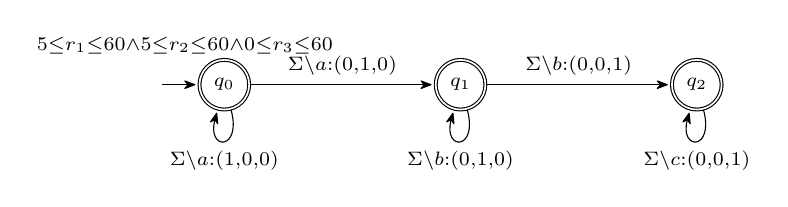
\begin{tikzpicture}[
  shorten >=1pt,node distance=3cm,on grid,>={Stealth[round]},
  initial text=, every state/.style={minimum size = 0.001cm},
  accepting text=$\scriptstyle5\leq r_1\leq 60\wedge 5\leq r_2\leq 60\wedge 0\leq r_3\leq 60$, 
  ]

  \node[state,initial, accepting]            (q_0)                      {$\scriptstyle q_0$};
  \node[state, accepting]                    (q_1) [right=of q_0]       {$\scriptstyle q_1$};
  \node[state, accepting]         (q_2) [right=of q_1]       {$\scriptstyle q_2$};
  \node at (-0.5,0.5) {$\scriptstyle5\leq r_1\leq 60\wedge 5\leq r_2\leq 60\wedge 0\leq r_3\leq 60$};

  \path[->] (q_0) edge node [above] {$\scriptstyle \Sigma \setminus a:(0,1,0)$} (q_1)
            (q_0) edge [loop below] node  {$\scriptstyle\Sigma \setminus a:(1,0,0)$} (q_0)
            (q_1) edge node [above] {$\scriptstyle\Sigma \setminus b:(0,0,1)$} (q_2)
            (q_1) edge [loop below] node  {$\scriptstyle\Sigma \setminus b:(0,1,0)$} (q_1)
            (q_2) edge [loop below] node  {$\scriptstyle\Sigma \setminus c:(0,0,1)$} (q_2);
\end{tikzpicture}

% \begin{tikzpicture}[
%   shorten >=1pt,node distance=2cm,on grid,>={Stealth[round]},
%   initial text=, every state/.style={minimum size = 0.001cm,
%       accepting text=$\scriptstyle 1\leq r_1\leq 100$, accepting/.style=accepting by arrow}
%   ]
%   \node[state,initial]            (q_0)                      {$q_0$};
%   \node[state]                    (q_1) [right=of q_0]       {$q_1$};
%   \node[state,accepting]          (q_2) [right=of q_1]       {$q_2$};

%   \path[->] (q_0) edge              node      [above]           {$\scriptstyle a:(1)$} (q_1)
%   (q_1) edge              node      [above]           {$\scriptstyle b:(0)$} (q_2)
%   (q_2) edge [bend left]  node      [below]           {$\scriptstyle\epsilon: (0)$} (q_0);
% \end{tikzpicture}


    \caption{An automaton recognizing the language of $(\Sigma \setminus a)^{\{5, 60\}} (\Sigma \setminus b)^{\{5, 60\}} (\Sigma \setminus c)^{\{0, 60\}}$}
    \label{fig:counting}
  \end{figure}
\end{example}
}
%%%%%%%%%%%%%%%%%%%%%%%%%%%%%%%%%%%%%%
%%%%%%%%%%%%%%%%%%%%%%%%%%%%%%%%%%%%%%

% Parikh's theorem \cite{parikh_theorem}\cite{parikh_anthony}\cite{parikh_compute} states that the Parikh image of a context-free language is semilinear so that it can be written as Presburger formula. Following the version for context-free grammar \cite{parikh_compute} and the version for regular expression \cite{parikh_for_nfa}, we define the Parikh image of language of an CEFA $\aut = (Q, \Sigma, \delta, q_I, F, R, \theta)$  as follows:
% \begin{table}[h]
%   \begin{tabular}{l l r}
%     $\psi(\aut)\equiv$& $\bigwedge\limits_{q\in Q}(\text{$f_q$ if $q\in F$ otherwise 0}) + \sum\limits_{(q,a,q',\myvec{v})\in\delta} t_{q,a,q',\myvec{v}} = $ & \\
%     & \quad \ \ (1 if $q = q_I$ otherwise 0) + $\sum\limits_{(q',a,q,\myvec{v})\in\delta} t_{q',a,q, \myvec{v}} $ & \\ 
%     & $\bigwedge\limits_{(q,a,q',\myvec{v})\in\delta} t_{q,a,q',\myvec{v}}\geq 0$ & (consistent formula)\\
%     & & \\
%     & $\bigwedge\limits_{(q,a,q',\myvec{v})\in\delta} t_{q,a,q',\myvec{v}}>0\rightarrow z_{q'} > 0$ & \\
%     & $\bigwedge\limits_{q\in F} z_q > 0\rightarrow f_q = 1$ & \\ 
%     & $\bigwedge\limits_{q\in Q} z_q > 0\rightarrow \bigvee\limits_{(q,a,q',\myvec{v})\in\delta} z_q = z_{q'} + 1\wedge t_{q,a,q',\myvec{v}}\geq 0 \wedge z_{q'} > 0$& (connected formula)\\
%     & & \\
%     &$\bigwedge\limits_{r_i\in R} r_i = \sum\limits_{(q,a,q',\myvec{v})\in \delta} t_{q,a,q',\myvec{v}}*\myvec{v}[i]$ & (register value formula)\\
%     & & \\
%     &$\bigwedge\limits_{q\in F} f_q > 0 \rightarrow \theta(q)$ & (accepting condition) 
%   \end{tabular}
% \end{table}
% $z_q$ is the distance of state $q$ from $q_f\in F$ in a spanning tree. $t_{q,a,q',\myvec{v}}$ represents the using times of transition $(q,a,q',\myvec{v})$ in the accepting run. $f_q$ stands for whether an accepting state $q\in F$ is the final state of a run. The Parikh image of $\aut$ is a Presburger formula $\psi(\aut)$, which is consistent and connected. The register value formula ensures \denghang{that} the register values are correctly updated regarding the accepting run. 
% \begin{example} \label{exapmle:parikh}
%   Suppose that we have a CEFA $\aut$ shown in Fig. \ref{subfig:aut_x}. Using $t_1, t_2, t_3$ to record the times of transitions in the accepting run of $\aut$, the Parikh image $\psi(\aut)$ is the quantifier-free Presburger formula $\psi_{cons}\wedge \psi_{conn} \wedge \psi_{val} \wedge \psi_{aut}$ where:
%   \begin{itemize}
%     \item $\psi_{cons} \equiv 1 = t_1 \wedge t_1 + t_3 = t_2 \wedge t_2 = t_3 + 1 \bigwedge\limits_{i\in[1,3]} t_i\geq 0$ is the consistent formula.
%     \item $\psi_{conn} \equiv \top $ is the connectivity formula because all transitions in $\aut$ are connected.
%     \item $\psi_{val} \equiv r_1=t_1 + t_3\wedge r_2 = t_1+t_2+t_3$ is the formula deciding the value of $r_1$ and $r_2$ after a run.
%     \item $\psi_{aut} \equiv r_2 = i\wedge 1 \leq r_1 \leq 100$ is the accepting condition of $\aut$.
%   \end{itemize}
%   $\psi(\aut)$ can be simplified to $t_3\geq 0 \wedge t_1=1\wedge r_1 = t_3 + 1\wedge r_2 = 2*t_3+2\wedge r_2=i\wedge 1\leq r_1\leq 100$. A possible solution is $t_1 =1, t_3 = 0, r_1=1, r_2=2$ and the corresponding accepted string $ab$. It is obvious that $r_1$ is the repeat times of $ab$ and $r_2$ is the length of $ab$.
% \end{example}
%\end{document}

%\vspace{-2mm}
\section{Solving RECL constraints} \label{sec:algorithm}
%\vspace{-2mm}
%!TEX root = ../main.tex
%\documentclass{standalone}
%\begin{document}

As mentioned in Section \ref{sec:overview}, the main idea of our approach is to model the counting operators symbolically by registers in automata, instead of unfolding them explicitly. Additionally, we represent string lengths using registers. This reduces the satisfiability of string constraints that involve regex-counting and string-length to the satisfiability of linear integer arithmetic, which can be solved by off-the-shelf SMT solvers. We also propose techniques to reduce automata sizes and utilize under approximations to enhance performance.
\subsection{Encode Regex-Counting to CEFA} \label{subsec:regex2cefa}
One key point of our approach is the encoding of counting operator. In this section, we define the construction of CEFA from the regular expression with counting. We divide the counting operator into \emph{handled} and \emph{non-handled}. The counting operator is called \emph{non-handled} if it is the sub-regex of other complement operator (e.g., $(\regex^{\{m,n\}})^C$), closure operator(e.g., $(\regex^{\{m,n\}})^*$), or counting operator (e.g., $(\regex^{\{m,n\}})^{\{m', n'\}}$), otherwise it is called \emph{handled}. A regex is called \emph{non-handled} if it contains any non-handled counting operators, and is called \emph{handled} otherwise.
% We must syntactically rewrite bounded repetition $\regex\{m,n\}$ if it is the sub-regex of complement (e.g., $(\regex\{m,n\})^C$), closure(e.g., $(\regex\{m,n\})^*$), and bounded repetition(e.g., $(\regex\{m,n\})\{m', n'\}$), we unwind it to $\regex^m\mid\cdots\mid\regex^n$. After this syntactic rewriting, we call the resulting regex $\regex'$ \emph{non-nested}.
Given a handled regex $\regex$, operations such as intersection, union, concatenation, complement, closure, and counting may appear. To construct the CEFA of $\regex$, we first create CEFA for each sub-regex and then combine them. Similar to the construction of NFA from regex\cite{aut_hopcraft}, our construction is inductive on the size of $\regex$. The base case is the construction for a single character, an empty string, or an empty language. The inductive step is the construction for the concatenation, union, intersection of two automata of sub-regexes, counting, closure, and complement of one automaton of sub-regex. We only discuss the inductive step for counting because it is the most important and the other operations are trivial. \newline
For a handled regular expression $\regex\{m,n\}$, suppose the CEFA recognizing $\regex$ is $\aut = (Q,\Sigma,\delta,q_I,F,\emptyset,\top)$, then the CEFA recognizing $\regex\{m,n\}$ is defined as $\aut_{m,n} = (Q, \Sigma, \delta',q_ I, F, r, \theta)$ where:
\begin{itemize}
  \item $r$ is a new register,
  \item $\delta'$ is composed by transition $q\xrightarrow[(0)]{a} q'$ for each transition $q\xrightarrow[()]{a} q' \in \delta$, and transition $q_f\xrightarrow[(1)]{\epsilon} q_I$ for each accepting state $q_f\in F$,
  \item $\theta$ is the function mapping each accepting state to a same linear integer arithmetic $m\leq r\leq n$.
\end{itemize}
The construction is illustrated in Fig.\ref{fig:construct_repetition}, where a new register $r$ is added to store the counting times. The transition $q\xrightarrow[(1)]{\epsilon} q_I$ is used to update the counting times for each $q\in F$. The accepting condition $\theta'$ constrains the counting times of the accepting word to the range $[m, n]$. 
\begin{figure}[h]
  \begin{subfigure}[b]{0.49\textwidth}
    \centering
    \begin{tikzpicture}[
      shorten >=1pt,node distance=2cm,on grid,>={Stealth[round]},
      initial text=, every state/.style={minimum size = 0.001cm},
      accepting text=$\top$, accepting/.style=accepting by arrow,
      ]

      \node[state,initial]            (q_0)                      {};
      \node[state, accepting]         (q_1) [right=of q_0]       {};
      \node [fit=(q_0) (q_1)] {$\cdots$};
    \end{tikzpicture}
    \caption{The CEFA recognizing $\regex$}
  \end{subfigure}
  \begin{subfigure}[b]{0.49\textwidth}
    \centering
    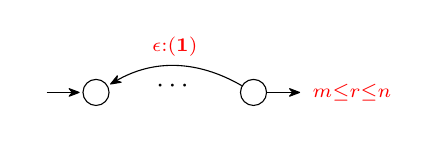
\begin{tikzpicture}[
      shorten >=1pt,node distance=2cm,on grid,>={Stealth[round]},
      initial text=, every state/.style={minimum size = 0.001cm},
      accepting text=\myemph{$\scriptstyle m\leq r\leq n$}, accepting/.style=accepting by arrow,
      ]

      \node[state,initial]            (q_0)                      {};
      \node[state, accepting]         (q_1) [right=of q_0]       {};
      \path[->] (q_1) edge[bend right]   node    [above] {\myemph{$\scriptstyle \mathbf{\epsilon:(1)}$}} (q_0);
      \node [fit=(q_0) (q_1)] {$\cdots$};
    \end{tikzpicture}
    \caption{The CEFA recognizing $\regex^{\{m,n\}}$}
  \end{subfigure}
  \caption{The construction of counting operator}
  \label{fig:construct_repetition}
\end{figure}
\begin{example}
  To construct the CEFA recognizing $(ab)\{1,100\}$. As shown in Fig.\ref{subfig:rep_aut_ab1_100}, the base cases are the constructions of character $a$ (Fig.\ref{subfig:rep_aut_a}) and $b$ (Fig.\ref{subfig:rep_aut_b}). The first inductive step is to concatenate them to one automaton (Fig.\ref{sub@subfig:rep_aut_ab}). The second inductive step is to add counting information on the automaton. To do that we add a new register $r_1$ and a transition $q_2\xrightarrow[(1)]{\epsilon} q_0$ to update the repetition times. The accepting condition in accepting state is $1\leq r_1\leq 100$ so that the counting time of the accepting word is in the range $[1,100]$. After that we get the CEFA recognizing $(ab)\{1,100\}$ shown in Fig.\ref{subfig:rep_aut_ab1_100}.
  \begin{figure}[h]
    \begin{subfigure}[b]{0.49\textwidth}
      \centering
      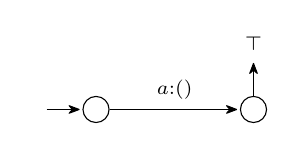
\begin{tikzpicture}[
        shorten >=1pt,node distance=2cm,on grid,>={Stealth[round]},
        initial text=, every state/.style={minimum size = 0.001cm},
        accepting text=$\scriptstyle \top$, accepting/.style=accepting by arrow,
        accepting where=above
        ]

        \node[state,initial]            (q_0)                      {};
        \node[state,accepting]                    (q_1) [right=of q_0]       {};

        \path[->] (q_0) edge              node      [above]           {$\scriptstyle a:()$} (q_1);
      \end{tikzpicture}
      \caption{The CEFA recognizing $a$}
      \label{subfig:rep_aut_a}
    \end{subfigure}
    \begin{subfigure}[b]{0.49\textwidth}
      \centering
      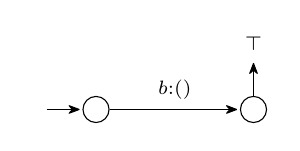
\begin{tikzpicture}[
        shorten >=1pt,node distance=2cm,on grid,>={Stealth[round]},
        initial text=, every state/.style={minimum size = 0.001cm},
        accepting text=$\scriptstyle \top$, accepting/.style=accepting by arrow,
        accepting where=above
        ]

        \node[state,initial]            (q_0)                      {};
        \node[state,accepting]                    (q_1) [right=of q_0]       {};

        \path[->] (q_0) edge              node      [above]           {$\scriptstyle b:()$} (q_1);
      \end{tikzpicture}
      \caption{The CEFA recognizing $b$}
      \label{subfig:rep_aut_b}
    \end{subfigure}
    \begin{subfigure}[b]{0.49\textwidth}
      \centering
      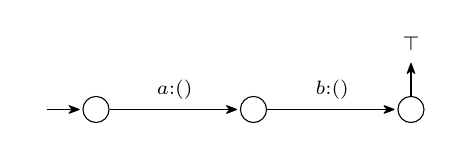
\begin{tikzpicture}[
        shorten >=1pt,node distance=2cm,on grid,>={Stealth[round]},
        initial text=, every state/.style={minimum size = 0.001cm},
        accepting text=$\scriptstyle\top$, accepting/.style=accepting by arrow,
        accepting where=above
        ]

        \node[state,initial]            (q_0)                      {};
        \node[state]                    (q_1) [right=of q_0]       {};
        \node[state, accepting]         (q_2) [right=of q_1]       {};

        \path[->] (q_0) edge              node      [above]           {$\scriptstyle a:()$} (q_1)
        (q_1) edge              node      [above]           {$\scriptstyle b:()$} (q_2);
      \end{tikzpicture}
      \caption{The CEFA recognizing $ab$}
      \label{subfig:rep_aut_ab}
    \end{subfigure}
    \begin{subfigure}[b]{0.49\textwidth}
      \centering
      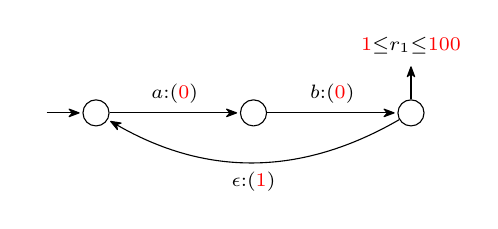
\begin{tikzpicture}[
        shorten >=1pt,node distance=2cm,on grid,>={Stealth[round]},
        initial text=, every state/.style={minimum size = 0.001cm},
        accepting text=$\scriptstyle\myemph{1}\leq r_1\leq\myemph{100}$, accepting/.style=accepting by arrow,
        accepting where=above
        ]

        \node[state,initial]            (q_0)                      {};
        \node[state]                    (q_1) [right=of q_0]       {};
        \node[state,accepting]          (q_2) [right=of q_1]       {};

        \path[->] (q_0) edge              node      [above]           {$\scriptstyle a:(\myemph{0})$} (q_1)
        (q_1) edge              node      [above]           {$\scriptstyle b:(\myemph{0})$} (q_2)
        (q_2) edge [bend left]  node      [below]           {$\scriptstyle \epsilon:(\myemph{1})$} (q_0);
      \end{tikzpicture}
      \caption{The CEFA recognizing $(ab)\{\myemph{1},\myemph{100}\}$}
      \label{subfig:rep_aut_ab1_100}
    \end{subfigure}
    \caption{The example of constructing regex with counting}
  \end{figure}
\end{example}
Above discusses the construction of counting operator in a handled regex. The counting operator of unhandled regex can not be constructed by the same way. For example, for an unhandled regex $(ab^{\{1,100\}})*$, there are infinite repetitions of regex $ab^{\{1,100\}}$. The counting times of each repetition are irrelevant, so that we can not represent them use finite registers. So we syntactically rewrite the unhandled counting operator into union operator and concatenation operator. More exactly, the sub-regex $\regex^{\{m,n\}}$ in the unhandled regex is rewritten into $\underbrace{\regex\cdot\regex\cdots\regex}_{m \text{ times}}\mid\cdots\mid \underbrace{\regex\cdot\regex\cdots\regex}_{n \text{ times}}$.
% Based on the decision procedure defined in the paper \cite{atva2020}, we propose an efficient algorithm to solve ESL formula $\varphi\wedge \psi$ where $\varphi$ is the conjunction of literals and $\psi$ is the conjunction of linear literals without length operation. For each string variable $x$, we first compute pre-images of all linear literal $i=|x|$. Then we generate CEFAs of all regular expressions $\regex$ in all regular literals $x\in \regex$ and intersect these CEFAs and pre-images to get the final automaton $\aut_x$ for $x$. At present, there is a final CEFA for each string variable $x$. The linear arithmetic constraint $\psi$ restricts the accepting word of final CEFAs. Thus the satisfiability problem is the emptiness checking problem of final CEFAs under $\psi$. If it is empty, the string constraints are unsatisfiable. Otherwise, the string constraints are satisfiable.
% The emptiness checking problem of CEFAs under linear integer arithmetic is theoretically pspace-complete\cite{atva2020}. To solve it efficiently for a practical example, we develop heuristic ways such as under-approximation (Section \ref{subsec:under-approx}) and symbolic-aware simplification (Section \ref{subsec:simplify}).
\subsection{Pre-iamge of String-length}
Given a string-length constraint, we build a CEFA with a register storing the length of accepted word. We call such a CEFA the \emph{pre-image} of it. Formally, the pre-image of length constraint is a CEFA $(\{q_I\}, \Sigma, \{q_I\xrightarrow[(1)]{\Sigma} q_I\}, q_I, \{q_I\}, r, \theta)$ where accpeting condition $\theta$ is based on the length value. For example, example \ref{eg:pre_len} shows the pre-image of length constraints $i=|x|$, in which $\theta(q_I)$ is $r = i$. This automaton contains a simple loop which increase $1$ on register $r$ for all char in $\Sigma$. So the accepting words of it is all words with length $i$. \newline
% The formal definition of pre-images of abundant string functions is listed in \cite{atva2020}, and we do not repeat it here.
\begin{example}[The pre-image of $i = |x|$]\label{eg:pre_len} 
  \begin{figure}[h]
    \centering
    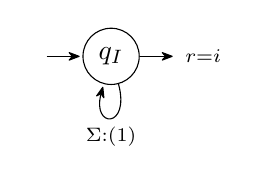
\begin{tikzpicture}[
      shorten >=1pt,node distance=2cm,on grid,>={Stealth[round]},
      initial text=, every state/.style={minimum size = 0.001cm},
      accepting text=$\scriptstyle{r=i}$, accepting/.style=accepting by arrow
      ]

      \node[state,initial,accepting]            (q_0)       {$q_I$};

      \path[->] (q_0) edge [loop below] node{$\scriptstyle\Sigma:(1)$} ();
    \end{tikzpicture}
  \end{figure}
\end{example} 
\subsection{Combine Regex-counting and String-length}
In the previous section, we have discussed the construction of regex-counting operator and the pre-image of string-length constraint. In this section, we show how to combine them to deal with the string constraints with regex-counting and string-length. 
\begin{definition} [The Product of Two CEFA]\newline
  Given two CEFAs $\aut_1 = (Q_1, \Sigma, \delta_1, q_{I_1}, F_1, R_1, \theta_1)$ and $\aut_2 = (Q_2, \Sigma, \delta_2, q_{I_2}, F_2, R_2, \theta_2)$ with $R_1\cap R_2 = \emptyset$, the product of them, denoted by $\aut_1 \times \aut_2$, is defined as $(Q_1\times Q_2, \Sigma, \delta, (q_{I_1}, q_{I_2}), F_1\times F_2, R_1\cup R_2, \theta)$ where
  \begin{itemize}
    \item $\delta$ comprises the tuples $((q_1, q_2), a, (q_1', q_2'), \myvec{v_1}\cdot \myvec{v_2})$ such that $(q_1, a, q_1', \myvec{v_1})\in \delta_1$ and $(q_2, a, q_2', \myvec{v_2})\in \delta_2$.
    \item $\theta((q_1, q_2))$ is $\theta_1(q_1)\wedge \theta_2(q_2)$ for each accepting state $(q_1, q_2)\in F_1\times F_2$.
  \end{itemize}
\end{definition}
With the help of product, we can combine the CEFAs of regex-counting and string-length. For example, the CEFA of string constraints $x\in \regex \wedge i=|x|$ is the product of the CEFA of $x\in \regex$ and the pre-image of $i=|x|$.

\subsection{Emptiness Checking Problem on CEFAs} \label{subsec:emptiness}
As mentioned, the emptiness checking problem of CEFAs under linear integer arithmetic $P$ is theoretically Pspace-complete. In our previous research  \cite{atva2020}, we rewrote CEFAs to an infinite system and used a model-checking tool \emph{nuXmv}\cite{nuxmv} to solve it. However, it needs to be more effective. So we put forward a new framework that brings in under-approximation and symbolic-aware simplification heuristics.\newline
As shown in Algorithm \ref{alg:emptiness}, we simplify the input CEFAs at line 1 because they may have many transitions and registers. The purpose of the simplification is to deal with duplication. After simplification, we try to find a solution by under-approximation at line 3 and line 4. An off-the-shelf SMT solver gives the result of $\varphi_{under}\wedge P$. If we find a solution, we return $false$ at line 5 because it implies that the CEFAs under linear integer arithmetic $P$ are not empty. Otherwise, we compute the Parikh images of the simplified CEFAs and check if the Parikh images are satisfiable in conjunction with $P$ at line 12. The Parikh image checking is complete so that satisfiability implies non-emptiness directly. \newline
The under-approximation program is executed many times until the $MaxBound$ is reached. $MaxBound$ is an empirical bound set to $15$ in our experiment because it brings exponential growth of searching space. The details of simplification are shown in Algorithm \ref{alg:simplify} and under-approximation are shown in Algorithm \ref{alg:underApprox}.\newline
\begin{algorithm}[h]
  \caption{ $\algfun{isEmpty}(auts, P)$}
  \label{alg:emptiness}
  \begin{algorithmic}[1]
    \Require the CEFAs $auts$ and the linear integer arithmetic $P$
    \Ensure $true$ or $false$
    \Statex
    \State $simpliAuts \leftarrow \algfun{simplify}(auts)$
    \For{$bound \gets 1, MaxBound$ }
    \State $\varphi_{under}\gets \algfun{underApprox}(simpliAuts, bound)$
    \If{$\varphi_{under}\wedge P$ is sat}
    \State \textbf{return} $false$
    \EndIf
    \EndFor
    \State $\varphi \gets \algfun{parikhImage}(simpliAuts)$
    \If{$\varphi\wedge P$ is unsat}
    \State \textbf{return} $true$
    \Else
    \State \textbf{return} $false$
    \EndIf
  \end{algorithmic}
\end{algorithm}
\subsubsection{Symbolic-Aware Simplification} \label{subsec:simplify}
The purpose of simplification is to remove duplicated transitions and registers. In the emptiness checking Algorithm \ref{alg:emptiness}, the vectors on the transitions are meritorious, while the letters are not. So we see the alphabet of the CEFA as unary (i.e., the alphabet is $\{a\}$) and see the vectors in the CEFA as letters in the NFA. The vector $\myvec{0}_n$ is seen as $\epsilon$. Precisely, given an CEFA $\aut = (Q, \Sigma, \delta, q_I, F, R, \theta)$, we obtain a symbolic form  $\aut_{sym} = (Q, \Sigma', \delta', q_I, F, R, \theta)$ where
\begin{itemize}
  \item $\Sigma' = \{a\}$,
  \item the transition set $\delta'$ is composed of transition $q\xrightarrow[\myvec{v}]{a}q'$ if there is a transition $q\xrightarrow[\myvec{v}]{b} q'$ in $\delta$ for $b\in \Sigma$ .
\end{itemize}
We directly apply algorithms of epsilon-closure, determination, and simplification in \cite{aut_hopcraft}. We see $q\xrightarrow[\myvec{0}_n]{a}q'$ as epsilon transition and compute the epsilon-closure based on it. We see $q\xrightarrow[\myvec{v}]{a}q'$ as a transition with label $(a, \myvec{v})$ and determine the automaton based on the label. Two accepting states are equivalent if they have the same accepting conditions, and two states are equivalent if they reach equivalent states for each label. We simplify the automaton by merging equivalent states.
The process above comprises line 3 and line 4 of Algorithm \ref{alg:simplify}. From line 5 to line 13, we check whether some registers are duplicated. (i.e., the values of these registers are always the same). If two registers $r_i$ and $r_j$ are duplicated at line 6, we remove one at line 7 and the corresponding update of vectors at line 9 to ensure the vectors are consistent with the new registers. After deleting the duplicated registers, we add constraint $r_i = r_j$ to store the value of the deleted register at line 11.
\begin{algorithm}[h]
  \caption{$\algfun{simplify}(auts)$}
  \label{alg:simplify}
  \begin{algorithmic}[1]
    \Require A set of CEFAs
    \Ensure The simplified CEFAs
    \Statex
    \For{$\aut \in auts$}
    \State Suppose that $\aut = (Q, \Sigma, \delta, q_I, F,
      R, \theta)$ and $R=(r_1,\cdots, r_n)$
    \State $\algfun{determinizeByVec}(\aut)$
    \State $\algfun{minimizeByVec}(\aut)$
    \ForAll{$(i, j)$ where $1\leq i \leq j \leq n$}
    \If {$\myvec{v}[i] = \myvec{v}[j]$ for every vector $\myvec{v}\in \aut$ }
    \State $R=(\cdots r_{j-1}r_{j+1}\cdots)$ \Comment remove $r_j$ from the register vector $R$
    \ForAll{$\myvec{v'}\in \aut$}
    \State $\myvec{v'}=(\cdots\myvec{v'}[j-1]\myvec{v'}[j+1]\cdots)$ \Comment remove $\myvec{v'}[j]$ from each vector $\myvec{v'}$
    \EndFor
    \State $\theta = \theta\wedge r_i = r_j$
    \EndIf
    \EndFor
    \EndFor
    \State \textbf{return} $auts$
  \end{algorithmic}
\end{algorithm}
\begin{example}
  Considering the CEFA recognizing $(a|b)\{1,100\}$ illustrated in Fig.\ref{subfig:simp_origin_cefa}. We first obtain a symbolic CEFA by using unary alphabet (Fig.\ref{subfig:simp_symbolic_cefa}) and then minimize it based on the symbolic label "$a/(1)$"(Fig.\ref{subfig:simp_final}).
  \begin{figure}[h]
    \begin{subfigure}[b]{0.49\textwidth}
      \centering
      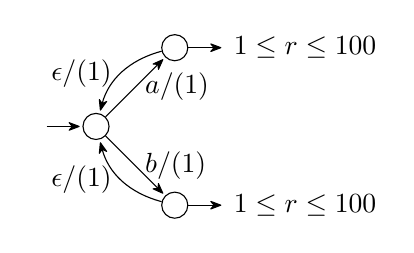
\begin{tikzpicture}[
        shorten >=1pt,node distance=1cm,on grid,>={Stealth[round]},
        initial text=, every state/.style={minimum size = 0.001cm},
        accepting text=$1\leq r \leq 100$, accepting/.style=accepting by arrow,
        ]

        \node[state,initial]            (q_0)                      {};
        \node         (q_tmp) [right=of q_0]       {};
        \node[state, accepting]         (q_1) [above=of q_tmp]       {};
        \node[state, accepting]         (q_2) [below=of q_tmp]       {};
        \path[->] (q_0) edge   node    [right] {$a/(1)$} (q_1)
        (q_0) edge   node    [right] {$b/(1)$} (q_2)
        (q_1) edge[bend right]   node    [left] {$\epsilon/(1)$} (q_0)
        (q_2) edge[bend left]   node    [left] {$\epsilon/(1)$} (q_0);
      \end{tikzpicture}
      \caption{The CEFA recognizing $(a|b)\{1,100\}$}
      \label{subfig:simp_origin_cefa}
    \end{subfigure}
    \begin{subfigure}[b]{0.49\textwidth}
      \centering
      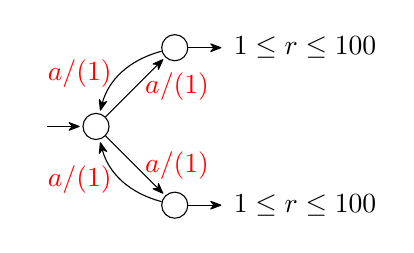
\begin{tikzpicture}[
        shorten >=1pt,node distance=1cm,on grid,>={Stealth[round]},
        initial text=, every state/.style={minimum size = 0.001cm},
        accepting text=$1\leq r \leq 100$, accepting/.style=accepting by arrow,
        ]

        \node[state,initial]            (q_0)                      {};
        \node         (q_tmp) [right=of q_0]       {};
        \node[state, accepting]         (q_1) [above=of q_tmp]       {};
        \node[state, accepting]         (q_2) [below=of q_tmp]       {};
        \path[->] (q_0) edge   node    [right] {$\myemph{a/(1)}$} (q_1)
        (q_0) edge   node    [right] {$\myemph{a/(1)}$} (q_2)
        (q_1) edge[bend right]   node    [left] {$\myemph{a/(1)}$} (q_0)
        (q_2) edge[bend left]   node    [left] {$\myemph{a/(1)}$} (q_0);
      \end{tikzpicture}
      \caption{The symbolic CEFA}
      \label{subfig:simp_symbolic_cefa}
    \end{subfigure}
    \begin{subfigure}[b]{0.49\textwidth}
      \centering
      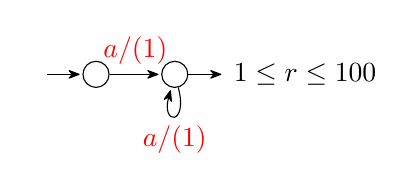
\begin{tikzpicture}[
        shorten >=1pt,node distance=1cm,on grid,>={Stealth[round]},
        initial text=, every state/.style={minimum size = 0.001cm},
        accepting text=$1\leq r \leq 100$, accepting/.style=accepting by arrow,
        ]

        \node[state,initial]            (q_0)                      {};
        \node[state, accepting]         (q_1) [right=of q_0]       {};
        \path[->] (q_0) edge   node    [above] {$\myemph{a/(1)}$} (q_1)
        (q_1) edge[loop below] node {$\myemph{a/(1)}$} (q_1);
      \end{tikzpicture}
      \caption{Simplify the CEFA based on symbolic label}
      \label{subfig:simp_final}
    \end{subfigure}
    \caption{Symbolic simplification removes duplicated transitions and states.}
    \label{fig:simplification_example}
  \end{figure}

\end{example}
\begin{example}
  Considering the string constraints $i=|x|\wedge j=|x|$. We compute the pre-images of $i=|x|$, $j=|x|$ and intersect these pre-images to get the final CEFA represented in Fig.\ref{subfig:duplicate}. However, the register $r_1$ and $r_2$ in the final CEFA are duplicated since their update functions are the same. We can simplify the CEFA by removing the duplicated register $r_2$ and corresponding update functions, as shown in Fig.\ref{subfig:remove_duplicate}. To maintain the value of $r_2$, we add a constraint $r_2=r_1$ to restrict the value of $r_2$ to be the same as $r_1$.
  \begin{figure}[h]
    \begin{subfigure}[b]{0.49\textwidth}
      \centering
      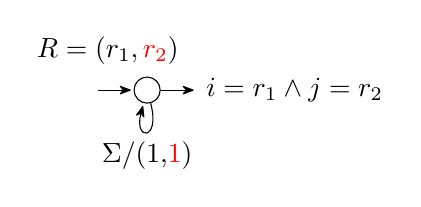
\begin{tikzpicture}[
        shorten >=1pt,node distance=1cm,on grid,>={Stealth[round]},
        initial text=, every state/.style={minimum size = 0.001cm},
        accepting text=${i=r_1\wedge j=r_2 }$, accepting/.style=accepting by arrow,
        ]
        \node at (-0.5,0.5) {$R=(r_1, \myemph{r_2})$};
        \node[state,initial,accepting]            (q_0)       {};

        \path[->] (q_0) edge [loop below] node{$\Sigma$/(1,\myemph{1})} ();
      \end{tikzpicture}
      \caption{An automaton with duplicated registers}
      \label{subfig:duplicate}
    \end{subfigure}
    \begin{subfigure}[b]{0.49\textwidth}
      \centering
      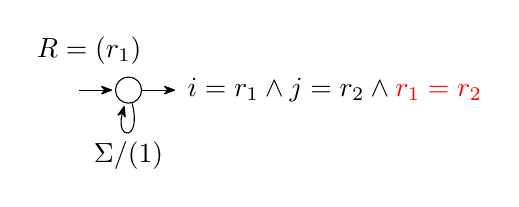
\begin{tikzpicture}[
        shorten >=1pt,node distance=1cm,on grid,>={Stealth[round]},
        initial text=, every state/.style={minimum size = 0.001cm},
        accepting text=${i=r_1\wedge j=r_2\wedge \myemph{r_1 = r_2} }$, accepting/.style=accepting by arrow,
        ]

        \node at (-0.5,0.5) {$R=(r_1)$};
        \node[state,initial,accepting]            (q_0)       {};

        \path[->] (q_0) edge [loop below] node{$\Sigma$/(1)} ();
      \end{tikzpicture}
      \caption{Remove the duplicated registers and corresponding update functions}
      \label{subfig:remove_duplicate}
    \end{subfigure}
    \caption{Symbolic simplification removes duplicated transitions and states.}
    \label{fig:duplicate}
  \end{figure}

\end{example}

\subsubsection{Under-Approximation} \label{subsec:under-approx}
An under-approximation procedure solves the satisfiable instances of the emptiness checking problem. Inspired by Bounded Model Checking \cite{bmc_1}\cite{bmc_2}\cite{bmc_3}, we explore the states of CEFA in typological order. We use string length as the bound and probe the CEFA from low to high bound. This section discusses the situation in which the string length bound is fixed. The main idea is to enumerate all possible runs ending in accepting states with lengths less than the fixed bound. Although the number of possible runs is an exponential growth of the bound, we usually solve practical satisfiable instances within 1s. As shown in the Algorithm \ref{alg:underApprox}, for each CEFA, we enumerate all runs whose length is less than the bound and compute the value of registers by the sum of vectors on the run at line 4. If the run is ended with an accepting state, then we compute the updates of registers by the sum of vectors on the run at line 6. Together with the accepting condition of the accepting state, we add the updates of registers to the under-approximation formula at line 7.
\begin{algorithm}[h]
  \caption{$\algfun{underApprox}(auts, bound)$}
  \label{alg:underApprox}
  \begin{algorithmic}[1]
    \Require The CEFAs $auts$ and string length $bound$
    \Ensure The linear integer arithmetic $\varphi_{under}$ representing under-approximation of the register values of $auts$
    \Statex
    \State $\varphi_{under} \gets false$
    \For{$\aut \in auts$}
    \State Suppose $\aut = (Q, \Sigma, \delta, q_I, F, (r_1, \cdots, r_m), \theta)$
    \ForAll{run $q_0q_1\cdots q_{n}$ whose length is less than $bound$}
    \If{$q_{n}\in F$}
    \State Let $\myvec{V}\leftarrow$ the sum of the vectors on the run
    \State $\varphi_{under} \gets \varphi_{under} \vee(\theta(q_n)\bigwedge\limits_{i\in[1,m]} r_i = \myvec{V}[i])$
    \EndIf
    \EndFor
    \EndFor
    \State \textbf{return} $\varphi_{under}$
  \end{algorithmic}
\end{algorithm}
\begin{example}
  Consider the automaton in Fig. \ref{subfig:aut_x} again. The solution of the Parikh image of it leads to a complete but inefficient result since the quantifier-free linear integer arithmetic formulas are solved in exponential time \cite{parikh_compute}. Under-approximation can accelerate the solving process. When we set the bound to 2, the under-approximation program will enumerate all runs whose length is 2. One of them is $q_I\xrightarrow[(1,1)]{a} q_1\xrightarrow[(0,1)]{b} q_f$. The corresponding registers' values are $r_1 = 1+0 = 1, r_2 = 1+1 = 2$. Checking for $r_1= 1\wedge r_2=2\wedge r_2=i\wedge 1\leq r_1\leq100$ is a lightweight process because the values of $r_1$ and $r_2$ are fixed.
\end{example}


\subsection{High-level algorithm}
\begin{algorithm}[h]
  \caption{High-level algorithm}
  \label{alg:high}
  \begin{algorithmic}[1]
    \Require Conjunction of literals $\varphi$ and conjunction of linear literals $\psi$
    \Ensure \emph{sat} or \emph{unsat}
    \Statex
    \State $finalAuts \leftarrow \emptyset$
    \ForAll{string variables $x$ occurring in $\varphi$}
    \State $\aut_{len} \leftarrow$ intersection of all pre-images of $i=|x|$ in $\varphi$
    \State $\aut_{regex} \leftarrow$ intersection of all CEFAs of $x \in \regex$ in $\varphi$
    \State $\aut_x \leftarrow$ intersection of $\aut_{len}$ and $\aut_{regex}$
    \State $\aut_{nfa} \leftarrow$ NFA form of $\aut_x$
    \If{$\aut_{nfa}$ is empty}
    \State \textbf{return} \emph{unsat}
    \EndIf
    \State $finalAuts \leftarrow finalAuts \cup \{\aut_x\}$
    \EndFor
    \If{$\algfun{isEmpty}(finalAuts, \psi)$ }
    \State \textbf{return} \emph{unsat}
    \Else
    \State \textbf{return} \emph{sat}
    \EndIf
  \end{algorithmic}
\end{algorithm}
The pseudocode presented in Algorithm \ref{alg:high} outlines the framework of our solving process. We construct the automata of all length operations occurring in the ESL conjunction $\varphi$ at line 3 and the automata of all regular memberships at line 4. In the following steps, we call an automaton to be \emph{final} if we will not operate it anymore. The set $finalAuts$ contains all final automata for all string variables and is initially empty at line 1. The intersection of $\aut_{len}$ and $\aut_{regex}$ at line 5 ensures the final automaton of $x$ reserves both length and regular information. At line 6, we compute an NFA form to throw unsat rapidly. An NFA form of CEFA is obtained by removing update functions and accepting conditions while maintaining graph structure. More exactly, given a CEFA $\aut = (Q,\Sigma, \delta, q_I, F, R, \theta)$, the NFA form of $\aut$ is $(Q, \Sigma, \delta', q_I, F)$ where $\delta'$ is composed of transition $q\xrightarrow[]{a} q'$ for $q\xrightarrow[\myvec{v}]{a} q'\in \delta$. It is obvious that the NFA form is an over-approximation of the CEFA, so that unsat is directly thrown if we find the NFA form is already empty at line 7. Sometimes the over-approximation is useful. For example, to solve the string constraint $x\in \Sigma_{/a}\{1,300\}\wedge x\in \Sigma^*a\Sigma^* $ which CVC5 has failed on, the NFA form is empty because there is no path to accepting states. \newline
After obtaining all final CEFAs of all string variables and their NFA forms are not empty, we check whether the final CEFAs are empty under the linear integer arithmetic $\psi$ at line 12. If they are empty under $\psi$, we return $unsat$. Otherwise, we return $sat$.


%\end{document}

%\vspace{-2mm}
\section{Experiments} \label{sec:implementation}
%\vspace{-2mm}
%!TEX root = ../main.tex
%\documentclass{standalone}
%\begin{document}
In this section, we list our experimental results. We first present the overall experiment results on RegCoL and AutomatArk benchmark suites. Then we present experiment results of the large-counting part and evaluate the simplification techniques. \denghang{The goal of our experiments is to answer the following questions:
\begin{itemize}
  \item [Q1:] Are our decision procedure more efficient than the state-of-the-art string constraint solvers on RECL constraints? (Sec \ref{subsec:overall_eval})
  \item [Q2:] Why our decision procedure is more efficient?(Sec \ref{subsec:large_bounds_eval})
  \item [Q3:] Are the size-reduction techniques practical?(Sec \ref{subsec:size_reduction_eval})
  \item [Q4:] How effective is the algorithm for solving the nonemptiness problem compared to the case that uses the nuXmv model checker? (Sec \ref{subsec:size_reduction_eval})
\end{itemize}
}

%This section presents the empirical evaluation of OstrichCEA, which is our implementation of the decision procedure introduced in Section \ref{sec:algorithm}. Our objective is to validate the effectiveness of the proposed techniques by evaluating our tool's correctness and efficiency compared to other solvers. Furthermore, we assess the efficacy of our heuristics by testing different configurations of the tool. We have implemented our encoding for counting with two heuristic algorithms on Ostrich+ \cite{atva2020}. The pre-image computation for concatenation, \verb|indexOf|, \verb|substring|, \verb|replaceAll|, \verb|reverse| and finite transducer remain unchanged. OstrichCEA is written in Scala and based on the SMT solver Princess\cite{princess}.

\vspace{-2mm}
\subsection{Benchmark Suites and Experiment Setup}\label{sec:bench}
\vspace{-1mm}

Our experiments utilize two benchmark suites, namely, \emph{RegCoL} and \emph{AutomatArk}. \denghang{Other industrial benchmarks suites are not utilized because they contains no counting operator.} There are 48,843 instances in total, and all benchmark instances are in the SMTLIB2 format.
Moreover, it turns out that only 5\% of regexes among the 48,843 instances are non-register-representable (see Section~\ref{subsec:regex2cefa}).

\medskip
\noindent
\emph{RegCoL benchmark suite.} There are 40,628 RECL instances in the RegCoL suite. These instances are generated by extracting regexes with counting operators from the open source regex library \cite{regex_lingua_franca,redos_lenka} and manually constructing a RECL constraint $x \in e \wedge x \in e_{sani} \wedge |x| > 10$ for each regex $e$,
where $e_{sani} \equiv \overline{\Sigma^*(<+ >+'+''+\&)\Sigma^*}$ is a regular expression that sanitizes all occurrence of special characters $<$, $>$, $'$, $''$, or $\&$. 
%The artificial construction is meaningful because the special characters are offensive. 
The expression $e_{sani}$ is introduced in view of the fact that these characters are usually sanitized in Web browsers to alleviate the XSS attacks \cite{malware_detection_3_kudzu,CCH_18}.
%We would like to remark that there are about 500,000 real-world regular expressions in \cite{regex_lingua_franca,redos_lenka} and regular expressions with counting operators occupy about 8\% of them. 
\vspace{-0.1mm}

\medskip
\noindent
\emph{AutomatArk benchmark suite.}
This benchmark suite is adapted from the AutomatArk suite \cite{z3str3re} by picking out the string constraints containing counting operators. We also add the length constraint $|x| > 10$ for each string variable $x$. There are 8,215 instances in the AutomatArk suite.
Note that the original AutomatArk benchmark suite \cite{z3str3re} includes 19,979 instances, which are conjunctions of regular membership queries generated out of regular expressions in \cite{automatark}.

\medskip
\noindent
\denghang{
\emph{Large-Bounds part.} This benchmark suite is composed of 1,969 problem instances with large counting bounds (greater than or equal to $50$) from RegCoL and AutomatArk benchmark suites.  
%regex with upper bound greater than 50 and generate a \emph{`large-counting'} benchmark suite (1,969 instances in total). 
Moreover, in order to test the performance of the solvers on string constraints with large length bounds as well, we increase the length bound to $200$, that is, $|x| > 200$.
}
%%%%%%%%%%%%%%%%%% the benchmark suite written by Denghang %%%%%%%%%%%
%%%%%%%%%%%%%%%%%% the benchmark suite written by Denghang %%%%%%%%%%%

\medskip
\noindent
\emph{Distribution of problem instances w.r.t. counting bounds. }
The distribution of problem instances w.r.t. the counting bounds in RegCoL and AutomatArk suites is shown in Fig~\ref{fig:count_distri}, where the $x$-axis represents the counting bound and the $y$-axis represents the number of problem instances whose maximum counting bound is equal to the value of the $x$-axis. 
%The upper bound is the number $n$ of regex $e^{\{m,n\}}, e^{\{n,n\}}$ and $e^{\{n,\infty\}}$ (which is equivalent to $e^{\{n,n\}}e^*$). 
From Fig~\ref{fig:count_distri}, we can see that while most problem instances contain only small bounds, there are still around 2,000  (about 4\%) of them using large counting bounds (i.e. greater than or equal to $50$).
%Although most upper bounds are small, about two thousand of them are still greater than 50. 

\medskip
\noindent
\emph{Experiment setup.}
All experiments are conducted on CentOS Stream release 8 with 4 Intel(R) Xeon(R) Platinum 8269CY 3.10GHz CPU cores and 190 GB memory. We use the \textsc{zaligvinder} framework \cite{zaligvinder_2021} to execute the experiments, with a timeout of 60s for each instance.


%%%%%%%%%%%%%%%%%% the benchmark suite written by Denghang %%%%%%%%%%%
%%%%%%%%%%%%%%%%%% the benchmark suite written by Denghang %%%%%%%%%%%
\hide{
  We conducted a comparison on four sets of benchmarks based on regex with
  counting operator, consisting of a total of 49,379 instances. We analyze all 19 developed benchmarks listed in \cite{zaligvinder_2021} and find that only \textbf{AutomatArk} benchmarks have regular membership with the counting operator. In total, almost 18\% of the instances we evaluated were sourced from published industrial benchmarks or other solver developers. The other instances are generated by ourselves with regular expressions from the real world. Each set of the benchmark is evenly divided into "large" and "small": the "large" set contains instances with large upper bounds of the counting operator (the sum of upper bounds is greater than 50), and "small" contains remaining instances. About 10\% of the benchmarks are in a "large" set. More details about the benchmarks are shown below.

  \subsubsection{AutomatArk} is the 8,751 instances generated by Berzish et al.\cite{z3str3re}. It is based on real-world regular expression queries from Loris D'Antoni\cite{automatark}. The origin set comprises two tracks, a simple and a hard track, with 19,979 instances. The simple track contains instances with a single regular expression membership constraint, whereas the hard track can hold up to five membership constraints for a single variable per instance. We extract 8,751 instances containing counting operators.

  \subsubsection{ReDos} is the set of 1,624 instances we generated. It is based on the ReDos-attacked regular expression collected by Lenka et al. For each regular expression, we generate an instance as the template (\ref{eq:template}) where $\regex$ is the regular expression. The regular membership predicate $x\not\in \Sigma^*(<\mid >\mid '\mid ''\mid \&)\Sigma^*$ sanitizes the input string $x$ to avoid the attack. The length lower bound is set to $20$ for the "small" set and $50$ for the "large" set.

  \subsubsection{RegexLib} is the set of 1,623 instances we generated similarly to the \textbf{ReDos} benchmark. It is based on the regular expressions collected by James C. Davis et al.\cite{regex_lingua_franca} from regex lib website\cite{regexlib}. The website is the Internet's first Regular Expression Library. Currently, it has indexed 4149 expressions from 2818 contributors around the world since 2001. We extracted 1,623 instances containing bounded repetition from 4149 instances. The length lower bound is set to $20$ for the "small" set and $50$ for the "large" set.

  \subsubsection{StackOverflow} is the 37381 instances we generated similarly to the \textbf{ReDos} benchmark. As the Regexlib benchmark, the real-world regex expressions are collected by James C. Davis et al.\cite{regex_lingua_franca} from StackOverflow website\cite{stackoverflow}. The website is a question-and-answer site for professional and enthusiast programmers. We extracted 37,381 instances containing bounded repetition from almost 500,000 instances. The length lower bound is set to $20$ for the "small" set and $50$ for the "large" set.
  \begin{equation} \label{eq:template}
    x\in \regex \wedge x\not\in \Sigma^*(<\mid >\mid '\mid ''\mid \&)\Sigma^*\wedge |x| > 50(or \ 20)
  \end{equation}
}
%%%%%%%%%%%%%%%%%% the benchmark suite written by Denghang %%%%%%%%%%%
%%%%%%%%%%%%%%%%%% the benchmark suite written by Denghang %%%%%%%%%%%

\vspace{-2mm}
\subsection{Overall Evaluation}\label{subsec:overall_eval}
\vspace{-1mm}

We evaluate the performance of $\ostrichrecl$ against the state-of-the-art string constraint solvers, including CVC5
%(version 1.0.5) 
\cite{cvc5}, Z3seq \cite{z3seq}, Z3str3
%(github commit 59e9c87) 
\cite{z3str3}, Z3str3RE \cite{z3str3re}, and OSTRICH
%(github commit 8297d8d) 
\cite{ostrich2023}, on RegCoL and AutomatArk benchmark suites.
% Z3-trau \cite{z3trau} is not evaluated because it does not support \verb|re.diff|, the language difference operator of regular expressions.  
%The experiments are designed to answer the following two research questions. 
%\begin{description}
%\item[Q1] Does OSTRICH$^{\rm RECL}$ solve RECL constraints more efficiently than the state-of-the-art string constraint solvers ?
%
%\item[Q2] Do the simplification and under-approximation techniques proposed in Section~\ref{sec:algorithm} indeed improve the performance ?
%\end{description}

% \medskip
% \noindent
% \emph{Overall evaluation.} 
The experiment results can be found in Table~\ref{tab:results_regcol}. Note that we take the result of CVC5 as the ground truth\footnote{Initially,  we used the majority vote of the results of the solvers as the ground truth. Nevertheless, on some problem instances, all the results of the three solvers in the Z3 family are wrong (after manual inspection), thus failing this approach on these instances.}, \denghang{and the results distinct to the ground truth are called \emph{soundness errors} in the result table.} We can see that $\ostrichrecl$ solves almost all 48,843 instances, except 182 of them, that is, it solves \textbf{48,662} instances correctly. The number is %3,994/2,272/24,577/12,832/1,091/7,092 
\textbf{3,908/1,111/12,838/2,306/2,396 more} than the number of instances solved by CVC5/Z3str3RE/Z3str3/Z3seq/OSTRICH respectively.
%      
%A soundness error is reported if the result of a solver for an instance is different from CVC5. 
% their results on some instances are inconsistent with the results of the other three solvers, i.e. CVC5, OSTRICH, and OSTRICH$^{\rm RECL}$.
%
Moreover, $\ostrichrecl$ is the second fastest solver, whose average time on each instance is close to the fastest solver Z3str3RE (\textbf{1.93s}/1.62s). \denghang{To answer \textbf{Q1}, \textbf{$\ostrichrecl$ is the second fastest solver on these benchmark suites, and it solves the most number of instances}.}

%
\begin{table}
  \vspace{-4mm}
  \centering
  \begin{subtable}{0.513\textwidth}
      \centering
      \import{tables}{table_regcol.tex}
      \caption{Overall evaluation, with timeout = 60 seconds.}
      \label{tab:results_regcol}
  \end{subtable}
  \begin{subtable}{0.477\textwidth}
      \centering
      \import{tables}{table_simp.tex}
      \caption{Evaluation of the size-reduction techniques, with timeout = 60 seconds.}
      \label{tab:results_simp}
  \end{subtable}
  \vspace{-2mm}
  \caption{Overall evaluation and the evaluation of the size-reduction techniques}
  \vspace{-8mm}
\end{table}
% \begin{table}[ht]
%   \vspace{-5mm}
%   \begin{center}
%     \import{tables}{table_regcol.tex}
%   \end{center}
%   \caption{Overall Experiment results, with timeout = 60 seconds}
%   \label{tab:results_regcol}
%   \vspace{-9mm}
% \end{table}

\subsection{Evaluation on problem instances with large bounds}\label{subsec:large_bounds_eval}
% \smallskip
% \noindent
% \emph{Evaluation on problem instances with large bounds.}
%
\sout{We extract the 1,969 problem instances with large counting bounds (greater than or equal to $50$) from the RegCoL and AutomatArk benchmark suites.  
%regex with upper bound greater than 50 and generate a \emph{`large-counting'} benchmark suite (1,969 instances in total). 
Moreover, in order to test the performance of the solvers on string constraints with large length bounds as well, we increase the length bound to $200$, that is, $|x| > 200$.}
%
\begin{figure}[ht]
  \centering
  \begin{subfigure}[t]{0.49\textwidth}
    \centering\vskip 0pt
    \includegraphics[width=1\textwidth]{counting_distribution.png}  
    \caption{Distribution of problem instances w.r.t. counting bounds}  
    \label{fig:count_distri}
  \end{subfigure}
  \hfill
  \begin{subfigure}[t]{0.49\textwidth}
    \centering\vskip 0pt
    \import{tables}{table_large_count.tex}
    \vspace{4.5mm}
    \caption{Experiment results on Large-Bounds part, with timeout = 60 seconds.}
    \label{fig:table_large_count}
  \end{subfigure}
  \vspace{-2mm}
  \caption{Distribution of counting bounds and experiment results for large bounds}
\vspace{-5mm}
\end{figure}


% \begin{table}[ht]
%   \vspace{-5mm}
%   \begin{center}
%     \import{tables}{table_large_count.tex}
%   \end{center}
%   \caption{Large-counting experiment, with timeout = 60 seconds}
%   \label{tab:results_simp}
%   \vspace{-9mm}
% \end{table}

We evaluate the performance of $\ostrichrecl$ on 1,969 instances of the Large-Bounds part. 
The experiment results are put in Fig~\ref{fig:table_large_count}. From the results, $\ostrichrecl$ solves \textbf{1,873} instances correctly, which is \textbf{947/278/563/637/523 more} than that solved by CVC5/Z3str3RE/Z3str3/Z3seq/OSTRICH respectively. Moreover, $\ostrichrecl$ is \textbf{ 6.79/2.88/2.61/5.27/3.95} times faster than CVC5/ Z3str3RE/Z3str3/Z3seq/OSTRICH respectively. \denghang{To answer \textbf{Q2}, we can see that $\ostrichrecl$ is far more efficient than the other solvers on problem instances with large bounds. \textbf{It is because the complexity in our decision procedure is irrelevant to counting bounds}, while the complexity of other solvers is linear or even exponential to counting bounds.}

\subsection{Evaluation of the effectiveness of size-reduction techniques}\label{subsec:size_reduction_eval}
% \medskip
% \noindent 
% \emph{Evaluation of the effectiveness of the automata size-reduction techniques.}
We also do experiments to evaluate the effectiveness of the automata size-reduction techniques, that is, Step 2 in Section~\ref{subsec:cefadec}. 
Let us use $\ostrichrecl_{\rm -SIMP}$ to denote $\ostrichrecl$ with the size-reduction techniques removed. 
Meanwhile, we compare $\ostrichrecl$ and $\ostrichrecl_{\rm -SIMP}$ against $\ostrichrecl_{\rm NUXMV}$, where the $\cefadec$ problem is solved by the \textsc{nuXmv} model checker \cite{nuxmv}, instead of the procedure in Section~\ref{subsec:cefadec}. 
The experiment results are put in Table~\ref{tab:results_simp}. 
%$\ostrichrecl_{\rm -SIMP}$ is the tool without simplification techniques. $\ostrichrecl_{\rm NUXMV}$ is the tool using \textsc{nuXmv}-based techniques. 
From the results, $\ostrichrecl$ solves \textbf{1,503 more} instances and is \textbf{2.21} times faster than $\ostrichrecl_{\rm -SIMP}$. \denghang{To answer \textbf{Q3}, \textbf{the size-reduction techniques indeed play a vital role in the performance improvement}}. Moreover, $\ostrichrecl$ solves \textbf{1,798 more} instances and is \textbf{3.13} times faster than $\ostrichrecl_{\rm NUXMV}$. \denghang{To answer \textbf{Q4}, \textbf{our algorithm for solving the nonemptiness problem is much better than the \textsc{nuXmv}-based techniques}}.

%Moreover, we encode the $\cefadec$ problem to an infinite state transition system and use \textsc{nuXmv}\cite{nuxmv} to solve it. We also compare the simplification techniques to the \textsc{nuXmv}-based techniques.
%$\ostrichrecl_{\rm NUXMV}$ is the tool using \textsc{nuXmv}-based techniques.
%We evaluate the simplification techniques by comparing the performance of $\ostrichrecl$ with and without the simplification techniques. 

% \begin{table}[ht]
%   \vspace{-5mm}
%   \begin{center}
%     \import{tables}{table_simp.tex}
%   \end{center}
%   \caption{Simplification technique evaluation, with timeout = 60 seconds}
%   \label{tab:results_simp}
%   \vspace{-9mm}
% \end{table}




% The results are in Table~\ref{tab:results_simplification}. We can see that the simplification technique improves the performance of $\ostrichrecl$ significantly. It solves 1,111 more instances and is 1.62 times faster than $\ostrichrecl$ without the simplification technique.

% \begin{table}[ht]
% %\vspace{-1mm}
% \begin{center}
%   \import{tables}{table_automatark.tex}
% \end{center}
%   \caption{Experiment results on AutomatArk, with timeout = 60 seconds}
%   \label{tab:results_automatark}
% \vspace{-6mm}
% \end{table}

% The experiment results on the AutomatArk benchmark suite are put in Table~\ref{tab:results_automatark}. 
% From Table~\ref{tab:results_automatark}, we can see that $\ostrichrecl$ solvers almost all 8,215 instances, except 39 of them, that is, it solves 8,176 instances correctly, which is %3,994/2,272/24,577/12,832/1,091/7,092 
% 101/191/4,094/2,632/9/1,587
% more than the number of instances solved by CVC5/Z3seq/Z3-Trau/Z3str3/Z3str3RE/OSTRICH respectively. 
% %    
% Still, the soundness errors are reported by taking the results of CVC5 as the ground truth.
%Note that Z3-Trau has soundness errors, where the result of CVC5 is taken as the ground truth. If CVC5 reports ``unknown'' or ``timeout'' in some instances, then no soundness errors will be reported in this instance. 
%A soundness error is reported if the result of a solver for an instance is different from CVC5. 
% their results on some instances are inconsistent with the results of the other three solvers, i.e. CVC5, OSTRICH, and OSTRICH$^{\rm RECL}$.
%
% Moreover, $\ostrichrecl$ spends 2.49 seconds per instance on average. 
%while the fastest solver Z3str3RE spends 1.71 seconds per instance, and the other solvers spend at least 3.49 seconds per instance.  
%Note that Z3-Trau reports ``unknown'' on 2,552 instances, which seems to be mainly attributed to the fact that it does not support \verb|re.diff|, the language difference operator of regular expressions. 

% In summary, $\ostrichrecl$ solves 48,698 out of 48,843 instances, 1,091 more than Z3str3RE, the state-of-the-art best solver on RECL constraints. Moreover, the speed of $\ostrichrecl$ is the second fastest and comparable to that of Z3str3RE. (See Table~\ref{tab:results_summary}.)

% \begin{table}[ht]
% \vspace{-3mm}
% \begin{center}
%   \import{tables}{table_summary.tex}
% \end{center}
%   \caption{Experiment results: A Summary}
%   \label{tab:results_summary}
% \vspace{-6mm}
% \end{table}


%Q1 is answered by running OSTRICH$^{\rm RECL}$ and the aforementioned solvers on AutomatArk and RegCoL. 

%\zhilin{may add the results for the two benchmark suites separately.}


%%%%%%%%%%%%%%%%%% Q2 removed %%%%%%%%%%%%
%%%%%%%%%%%%%%%%%% Q2 removed %%%%%%%%%%%%
\hide{
  \begin{table}[ht]
    \vspace{-3mm}
    \begin{center}
      \subimport{tables}{table_heuristic.tex}
    \end{center}
    \caption{Experiment results for Q2, where the timeout period is 60 seconds}
    \label{tab:results_heuristics}
    \vspace{-6mm}
  \end{table}

  To answer Q2, we compare OSTRICH$^{\rm RECL}$ with its three variants, namely, OSTRICH$^{\rm RECL}$ where the simplification, under-approximation, or both are removed.
  For convenience, let us use OSTRICH$^{\rm RECL^-}$ to denote the variant of OSTRICH$^{\rm RECL}$ that both simplification and under-approximation techniques are removed,
  OSTRICH$^{\rm RECL^-}_{+\rm SR}$ (resp. OSTRICH$^{\rm RECL^-}_{+\rm UA}$) to denote the variant that is obtained by adding the simplification (resp. under-approximation) techniques to OSTRICH$^{\rm RECL^-}$.
  %OSTRICH$^{\rm RECL}_{\rm -SR}$, OSTRICH$^{\rm RECL}_{\rm -UA}$, OSTRICH$^{\rm RECL}_{\rm -SRUA}$, which remove simplification, under-approximation, and both from OSTRICH$^{\rm RECL}$ respectively. 
  The experiment results can be found in Table~\ref{tab:results_heuristics}.
  From Table~\ref{tab:results_heuristics}, we can see that adding simplification techniques help to solve 1,563 more instances and reduce the average time per instance for 46.4\% (see the OSTRICH$^{\rm RECL^-}_{\rm +SR}$ column), while adding under-approximation techniques help to solve 1,476 more instances and reduce the average time per instance for 42.7\% (see the OSTRICH$^{\rm RECL^-}_{\rm +UA}$ column), moreover, adding both help to solve 1,579 more instances and reduce the average time per instance for 46.5\% (see the OSTRICH$^{\rm RECL}$ column). Note that adding under-approximation to OSTRICH$^{\rm RECL^-}_{\rm +SR}$ helps to solve 19 more sat instances while reducing the number of solved unsat instances by 3 since under approximation techniques do not help to solve unsat instances.
}
%%%%%%%%%%%%%%%%%% Q2 removed %%%%%%%%%%%%
%%%%%%%%%%%%%%%%%% Q2 removed %%%%%%%%%%%%
%Moreover, adding these techniques also decrease the average time spent in solving each instance considerably.


%\zhilin{stopped here}

%%%%%%%%%% original texts by denghang %%%%%%%%%
%%%%%%%%%% original texts by denghang %%%%%%%%%
\hide{
  %
  We have evaluated OstrichCEA compared to five other prominent string solvers currently available. We evaluate the solvers by directly comparing the number of cases correctly solved, the average time taken with and without timeouts, and the total count of soundness errors and program crashes. One of these solvers is CVC5\cite{cvc5}, a general SMT solver that uses algebraic reasoning to handle strings and regular expressions and is the winner of SMT-COMP 2022\cite{smt-comp}. Another solver, Z3str3\cite{z3str3}, is the most recent edition we can get to the Z3-str family and utilizes a word equation reduction approach to reason about regular expressions. Z3str3RE\cite{z3str3re} is a variant of Z3str3 that incorporates length-aware algorithms and heuristics. Z3seq\cite{z3seq} is a sequence solver which uses a novel derivative theory for solving extended regular expressions. Z3-Trau\cite{z3trau} is the Z3 version of trau\cite{trau} that employs a flat automata-based approach, incorporating both under- and over-approximations. Ostrich\cite{Ostrich} is the tool we extend which uses automaton to model the semantics of string functions and regular memberships. We used the 1.0.5 binary version of CVC5, commit 59e9c87 of Z3str3, the last version of Z3str3RE, 4.8.9 binary version of Z3Seq, commit 1628747 of Z3-Trau and commit 8297d8d of Ostrich. Z3-Trau does not support \verb|re.diff|. All other solvers support all syntax sugars listed in SMT-LIB standard\cite{smt_lib}. We omitted Z3str4\cite{z3str4} because the provided reproduction package link is wrong. All experiments are conducted on CentOS Stream release 8 with 12 Intel(R) Xeon(R) Platinum 8269CY CPU T 3.10GHz processors and 190 GB memory. We used Zaligvinder\cite{zaligvinder_2021} framework and set the timeout to 60 seconds.

  %\subsection{Overall Evaluation}
  In Fig.\ref{fig:cactus_all}, the cactus plot illustrates the cumulative time each solver takes for all cases in ascending order of runtime. Solvers located towards the right and lower portion of the plot indicate better performance. \newline
  Table \ref{tab:results_all} summarizes the results demonstrating OstrichCEA's superior performance, solving the most significant number of instances and outperforming most competing solvers. Including timeouts, OstrichCEA is \textbf{1.52}\mult{} faster than Z3Seq, \textbf{2.23}\mult{} faster than Ostrich, \textbf{2.26}\mult{} faster than Z3-Trau, \textbf{3.08}\mult{} faster than Z3str3, \textbf{3.11}\mult{} faster than CVC5 and close to Z3str3RE with \%2 speed loss . Note that CVC5\cite{cvc5} yielded 5370 timeouts(11\% of all instances), and Z3str3\cite{z3str3} yielded 6139 timeouts(12\% of all instances), which is much more than other solvers. Both CVC5 and Z3str3 are DPLL(T)-based solvers. It seems that almost 10\% of the benchmarks we used seem unsuitable for them. Z3-trau\cite{z3trau} yielded 21,152 unknowns because it does not support \verb|re.diff|. Z3-trau\cite{z3trau} yielded 6673 crashes (13\% of the instances) and 1233 soundness errors (2\% of the instances), which is a large portion. Z3-based solvers Z3str3 yielded 38 soundness errors, Z3seq\cite{z3seq} yielded 51 soundness errors and Z3str3RE\cite{z3str3re} yielded 39 soundness error. Most of them are due to the mistake of formalization of the backslash character. OstrichCEA resulted in 5 unknowns because it reached the maximum threshold of limited memory 2GB. More details of the results of each benchmark are shown in \ref{appendix:experiential_results}.
  \begin{figure}[h]
    \centering
    \import{figures}{cactus_plot_all.tex}
    \caption{Cactus plot summarizing performance on all benchmarks.}
    \label{fig:cactus_all}
  \end{figure}

  %\subsection{Analysis of Individual Heuristics}
  In order to demonstrate the efficacy of the individual heuristics outlined in Section \ref{sec:algorithm} and incorporated into OstrichCEA, we assessed various tool configurations in which one or more heuristics were disabled. Figure \ref{fig:cactus_heuristics} and Table \ref{tab:results_heuristics} display the outcomes. The "OstrichCEA" plot line represents the tool's performance when all heuristics are enabled, while the "All heuristics off" line represents performance when all heuristics are disabled. The remaining plot lines exhibit performance with only the named heuristic disabled while all others are enabled. The plots and table show that OstrichCEA functions most effectively when all heuristics are enabled. In average time with timeout times, OstrichCEA performs \textbf{1.78}$\times$ faster than employing none of our heuristics, \textbf{1.37}$\times$ faster than turning off simplification, \textbf{1.15}$\times$ faster than truing off under-approximation.
  \begin{figure}
    \subimport{figures/}{cactus_plot_heuristic.tex}
    \caption{A performance comparison was made on all benchmarks by turning off individual heuristics using a cactus plot.}
    \label{fig:cactus_heuristics}
  \end{figure}
  \begin{table}
    \subimport{tables}{table_heuristic.tex}
    \caption{A performance comparison was made on all benchmarks by turning off individual heuristics.}
    \label{tab:results_heuristics}
  \end{table}
}
%%%%%%%%%% original texts by denghang %%%%%%%%%
%%%%%%%%%% original texts by denghang %%%%%%%%%
%\end{document}

%\vspace{-2mm}
\section{Conclusion} \label{sec:conclu}
%\vspace{-2mm}
%!TEX root = ../main.tex
%\documentclass{standalone}
%\begin{document}

%TODO
This work proposes an efficient automata-theoretical approach for solving RECL constraints, that is, string constraints with regex-counting and string-length. The approach is based on the idea of encoding counting operators in regular expressions by registers symbolically, instead of unfolding them explicitly. Moreover, this paper proposes an automata-size reduction technique and an under-approximation based solution searching technique to improve the performance. Finally, we use two benchmark suites comprising 48,834 instances in total to evaluate the performance of our approach. The experimental results show that our approach can solve more instances than the state-of-the-art best solvers on RECL constraints, with a comparable performance. For the future work, we plan to investigate symbolic approaches to dealing with nested counting operators. 

%This paper aims to efficiently solve the string constraints with bounded repetition and linear integer constraints on string length. The bounded repetition is encoded by an automaton model CEFA whose size is linear to the bound. Moreover, we extend the algorithm in the paper \cite{atva2020} with heuristics such as under-approximation and symbolic-aware simplification. The implementation of the algorithm is done on string solver OstrichCEA. The extensive empirical comparison against state-of-art string solvers over a large and diverse benchmark shows the power of our encoding for bounded repetition and heuristic ways. In the future, we plan to explore how to solve nested repetition and use CEFA to solve more string operations.



%\end{document}

\newpage

%%
%% The next two lines define the bibliography style to be used, and
%% the bibliography file.
\bibliographystyle{splncs04}
\bibliography{ref}

%\appendix
%\section{Encoding Other Operations to CEFA} \label{appendix:cefa}

\subsection{Concatenation}\label{subsec:con}
Given two CEFAs $\aut_1 = (Q_1, \Sigma, \delta_1, q_{I_1}, F_1, R_1, \theta_1)$ and $\aut_2 = (Q_2, \Sigma, \delta_2, q_{I_2}, F_2, R_2, \theta_2)$ with $R_1\cap R_2= \emptyset$ and $|R_1|=m,|R_2|=n$, the concatenation of them is defined as $\aut_{\cdot}=(Q_1\cup Q_2, \Sigma, \delta', q_{I_1}, F_2, R_1\cdot R_2, \theta_1\wedge\theta_2)$ where $\delta'$ is composed by
\begin{itemize}
  \item $q_1\xrightarrow[\myvec{v_1}\cdot 0_n]{a} q_1'$ for each transition $q_1\xrightarrow[\myvec{v_1}]{a} q_1' \in \delta_1$,
  \item $q_2\xrightarrow[0_m\cdot\myvec{v_2}]{a} q_2'$ for each transition $q_2\xrightarrow[\myvec{v_2}]{a} q_2' \in \delta_2$,
  \item and $q_1\xrightarrow[0_{m+n}]{\epsilon} q_{I_2}$ for each $q_1\in F_1$.
\end{itemize}
\begin{figure}[h]
  \centering
  \begin{subfigure}[h]{0.3\textwidth}
    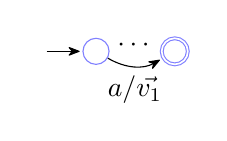
\begin{tikzpicture}[shorten >=1pt,node distance=1cm,on grid,>={Stealth[round]},
      every state/.style={draw=blue!50,minimum size = 0.1cm}, initial text=]
      \node[state, initial]   (q_0) {};
      \node[state, accepting]    (q_1) [right=of q_0] {};
      \path[->] (q_0) edge [bend right] node [below] {$a/\myvec{v_1}$} (q_1);
      \node [fit=(q_0) (q_1)] {$\cdots$};
    \end{tikzpicture}
    \caption{The CEFA $\aut_1$}
  \end{subfigure}
  \begin{subfigure}[h]{0.3\textwidth}
    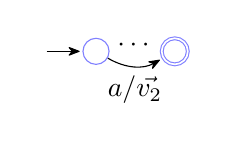
\begin{tikzpicture}[shorten >=1pt,node distance=1cm,on grid,>={Stealth[round]},
      every state/.style={draw=blue!50,minimum size = 0.1cm}, initial text=]
      \node[state, initial]   (q_0) {};
      \node[state, accepting]    (q_1) [right=of q_0] {};
      \path[->] (q_0) edge [bend right] node [below] {$a/\myvec{v_2}$} (q_1);
      \node [fit=(q_0) (q_1)] {$\cdots$};
    \end{tikzpicture}
    \caption{The CEFA $\aut_2$}
  \end{subfigure}
  \begin{subfigure}[h]{0.3\textwidth}
    \centering
    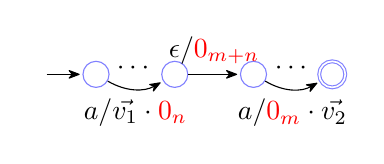
\begin{tikzpicture}[shorten >=1pt,node distance=1cm,on grid,>={Stealth[round]},
      every state/.style={draw=blue!50,minimum size = 0.1cm}, initial text=]
      \node[state, initial]   (q_0) {};
      \node[state]    (q_1) [right=of q_0] {};
      \node[state]    (q_2) [right=of q_1] {};
      \node[state, accepting]    (q_3) [right=of q_2] {};
      \path[->]
      (q_0) edge [bend right] node [below] {$a/\myvec{v_1}\cdot \red{0_n}$} (q_1)
      (q_1) edge node [above] {$\epsilon/\red{0_{m+n}}$} (q_2)
      (q_2) edge [bend right] node [below] {$a/\red{0_m}\cdot \myvec{v_2}$} (q_3);
      \node [fit=(q_0) (q_1)] {$\cdots$};
      \node [fit=(q_2) (q_3)] {$\cdots$};
    \end{tikzpicture}
    \caption{The concatenation of $\aut_1$ and $\aut_2$}
  \end{subfigure}
  \caption{Concatenation}
  \label{fig:con}
\end{figure}
The concatenation of two CEFAs is similar to that of two NFAs, except that the registers and their updates are also concatenated.

Figure \ref{fig:con} outlines the vector change on transitions when concatenating two CEFA. Without losing information, $\aut_{\cdot}$ contains all registers in $\aut_1$ and $\aut_2$. Furthermore, $\aut_{\cdot}$ update registers' value of $\aut_1$ and $\aut_2$ separately: $\aut_{\cdot}$ only update registers of $R_1$ on the transitions of $\aut_1$ and update registers of $R_2$ on the transition of $\aut_2$. $\theta'$ is the conjunction of $\theta_1$ and $\theta_2$ to make sure all linear constraints in $\aut_1$ and $\aut_2$ are satisfiable.
\subsection{Intersection}\label{subsec:inter}
Given two CEFAs $\aut_1 = (Q_1, \Sigma, \delta_1, q_{I_1}, F_1, R_1, \theta_1)$ and $\aut_2 = (Q_2, \Sigma, \delta_2, q_{I_2}, F_2, R_2, \theta_2)$ with $R_1\cap R_2 = \emptyset$, the intersection of them is defined as $\aut_{\times} = (Q_1\times Q_2, \Sigma, \delta', q_{I_1}\times q_{I_2}, F_1\times F_2, R_1\cdot R_2, \theta_1\wedge \theta_2)$ where $\delta'$ is composed by
\begin{itemize}
  \item transitions $(q_1,q_2)\xrightarrow[\myvec{v_1}\cdot\myvec{v_2}]{a} (q_1',q_2')$ if transition $q_1\xrightarrow[\myvec{v_1}]{a}q_1'$ and transition $q_2\xrightarrow[\myvec{v_2}]{a}q_2'$ exist individually in  $\delta_1$ and $\delta_2$.
\end{itemize}
\begin{figure}[h]
  \centering
  \begin{subfigure}[h]{0.30\textwidth}
    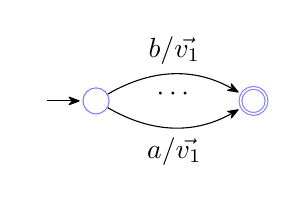
\begin{tikzpicture}[shorten >=1pt,node distance=2cm,on grid,>={Stealth[round]},
      % every fit/.style={draw,minimum height=2cm,minimum width=3.5cm,dashed},
      every state/.style={draw=blue!50,minimum size = 0.1cm}, initial text=]
      \node[state, initial]   (q_0) {};
      \node[state, accepting]    (q_1) [right=of q_0] {};
      \path[->]
      (q_0) edge [bend right] node [below] {$a$/$\myvec{v_1}$} (q_1)
      (q_0) edge [bend left] node [above] {$b$/$\myvec{v_1}$} (q_1);
      \node [fit=(q_0) (q_1)] {$\cdots$};
    \end{tikzpicture}
    \caption{The CEFA $\aut_1$}
  \end{subfigure}
  \begin{subfigure}[h]{0.30\textwidth}
    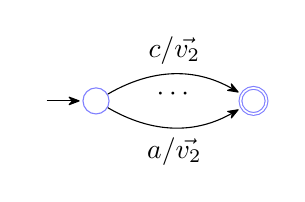
\begin{tikzpicture}[shorten >=1pt,node distance=2cm,on grid,>={Stealth[round]},
      % every fit/.style={draw,minimum height=2cm,minimum width=3.5cm,dashed},
      every state/.style={draw=blue!50,minimum size = 0.1cm}, initial text=]
      \node[state, initial]   (q_0) {};
      \node[state, accepting]    (q_1) [right=of q_0] {};
      \path[->]
      (q_0) edge [bend right] node [below] {$a$/$\myvec{v_2}$} (q_1)
      (q_0) edge [bend left] node [above] {$c$/$\myvec{v_2}$} (q_1);
      \node [fit=(q_0) (q_1)] {$\cdots$};
    \end{tikzpicture}
    \caption{The CEFA $\aut_2$}
  \end{subfigure}
  \begin{subfigure}[h]{0.3\textwidth}
    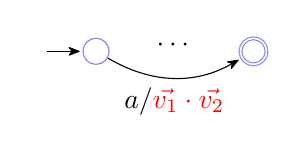
\begin{tikzpicture}[shorten >=1pt,node distance=2cm,on grid,>={Stealth[round]},
      % every fit/.style={draw,minimum height=2cm,minimum width=3.5cm,dashed},
      every state/.style={draw=blue!50,minimum size = 0.1cm}, initial text=]
      \node[state, initial]   (q_0) {};
      \node[state, accepting]    (q_3) [right=of q_0] {};
      \path[->]
      (q_0) edge [bend right] node [below] {$a$/\red{$\myvec{v_1}\cdot \myvec{v_2}$}} (q_3);
      \node [fit=(q_0) (q_3)] {$\cdots$};
    \end{tikzpicture}
    \caption{The intersection of $\aut_1$ and $\aut_2$}
  \end{subfigure}
  \caption{Intersection}
  \label{fig:inter}
\end{figure}
The intersection of two CEFAs is similar to that of NFA, except that the vectors and linear arithmetic are also intersected.

\subsection{Union}\label{subsec:union}
Given two CEFAs $\aut_1 = (Q_1, \Sigma, \delta_1, q_{I_1}, F_1, R_1, \theta_1)$ and $\aut_2 = (Q_2, \Sigma, \delta_2, q_{I_2}, F_2, R_2, \theta_2)$ with $R_1\cap R_2 = \emptyset$ and $|R_1|=m,|R_2|=n$, the union of them is defined as $\aut_{+} = (Q_1\cup Q_2\cup\{q_0\}, \Sigma, \delta', \{q_I\}, F_1\cup F_2, R_1\cdot R_2\cdot (r_1, r_2), \theta')$ where $\delta'$ is composed by
\begin{itemize}
  \item transitions $q_I\xrightarrow[0_{m+n}\cdot(1,0)]{\epsilon}q_1$ for all $q_1\in I_1$,
  \item transitions $q_I\xrightarrow[0_{m+n}\cdot(0,1)]{\epsilon}q_2$ for all $q_2\in I_2$,
  \item transitions $q_1\xrightarrow[\myvec{v_1}0_{n+2}]{a} q_1'$ for all $q_1\xrightarrow[\myvec{v_1}]{a} q_1'\in \delta_1$,
  \item transitions $q_2\xrightarrow[0_m\myvec{v_2}0_2]{a} q_2'$ for all $q_2\xrightarrow[\myvec{v_2}]{a} q_2'\in \delta_2$.
\end{itemize}
$r_1$ and $r_2$ are new registers to determine which automaton to run. $q_I$ is a new state where $q_I\not\in Q_1$ and $q_I\not\in Q_2$. Assume that basic determining formula $\theta$  is $(r_1>0\wedge\theta_1)\vee(r_2>0\wedge\theta_2)$, $\theta'$ is constructed differently in four cases:
\begin{itemize}
  \item $q_{I_1}\in F\wedge q_{I_2}\in F$: $\theta'$ = $\theta $;
  \item $q_{I_1}\in F\wedge q_{I_2}\not\in F$: $\theta'$ = $\theta \vee (r_1==0\wedge r_2==0\wedge\theta_1)$;
  \item $q_{I_1}\not\in F\wedge q_{I_2}\in F$: $\theta'$ = $\theta \vee (r_1==0\wedge r_2==0\wedge\theta_2)$;
  \item $q_{I_1}\in F\wedge q_{I_2}\in F$: $\theta'$ = $\theta \vee (r_1==0\wedge r_2==0\wedge(\theta_1\vee\theta_2))$;
\end{itemize}

\begin{figure}[h]
  \centering
  \begin{subfigure}{0.20\textwidth}
    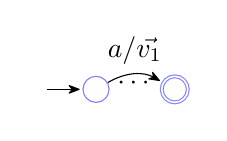
\begin{tikzpicture}[shorten >=1pt,node distance=1cm,on grid,>={Stealth[round]},
      % every fit/.style={draw,minimum height=2cm,minimum width=3.5cm,dashed},
      every state/.style={draw=blue!50,minimum size = 0.1cm}, initial text=]
      \node[state, initial]   (q_0) {};
      \node[state, accepting]    (q_1) [right=of q_0] {};
      \path[->]
      (q_0) edge [bend left] node [above] {$a$/$\myvec{v_1}$} (q_1);
      \node [fit=(q_0) (q_1)] {$\cdots$};
    \end{tikzpicture}
    \caption{The CEFA $\aut_1$}
  \end{subfigure}
  \begin{subfigure}{0.20\textwidth}
    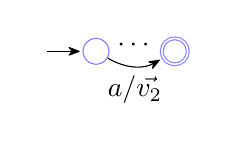
\begin{tikzpicture}[shorten >=1pt,node distance=1cm,on grid,>={Stealth[round]},
      % every fit/.style={draw,minimum height=2cm,minimum width=3.5cm,dashed},
      every state/.style={draw=blue!50,minimum size = 0.1cm}, initial text=]
      \node[state, initial]   (q_0) {};
      \node[state, accepting]    (q_1) [right=of q_0] {};
      \path[->]
      (q_0) edge [bend right] node [below] {$a$/$\myvec{v_2}$} (q_1);
      \node [fit=(q_0) (q_1)] {$\cdots$};
    \end{tikzpicture}
    \caption{The CEFA $\aut_2$}
  \end{subfigure}
  \begin{subfigure}{0.4\textwidth}
    \centering
    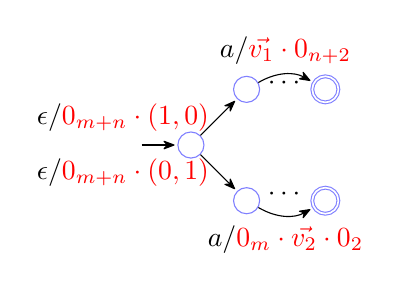
\begin{tikzpicture}[shorten >=1pt,node distance=1cm,on grid,>={Stealth[round]},
      % every fit/.style={draw,minimum height=2cm,minimum width=3.5cm,dashed},
      every state/.style={draw=blue!50,minimum size = 0.1cm}, initial text=]
      \node[state, initial]   (q_0) {};
      \node[state]   (q_1) [above right=of q_0] {};
      \node[state, accepting]   (q_1') [right=of q_1] {};
      \node[state]   (q_2) [below right=of q_0] {};
      \node[state, accepting]   (q_2') [right=of q_2] {};
      \path[->]
      (q_0) edge node [left] {$\epsilon/\red{0_{m+n}\cdot(1,0)}$} (q_1)
      (q_0) edge node [left] {$\epsilon/\red{0_{m+n}\cdot(0,1)}$} (q_2)
      (q_1) edge [bend left] node [above] {$a$/\red{$\myvec{v_1}\cdot 0_{n+2}$}} (q_1')
      (q_2) edge [bend right] node [below] {$a$/\red{$0_m\cdot \myvec{v_2}\cdot 0_2$}} (q_2');
      \node [fit=(q_1) (q_1')] {$\cdots$};
      \node [fit=(q_2) (q_2')] {$\cdots$};
    \end{tikzpicture}
    \caption{The union of $\aut_1$ and $\aut_2$}
  \end{subfigure}
  \caption{Union}
  \label{fig:union}
\end{figure}
To simulate the semantics of the union, we add transitions from $q_I$ to initial states of $\aut_1$ and $\aut_2$ to choose one automaton randomly. $r_1 > 0$ indicates we choose $\aut_1$ to run while $r_2 > 0$ indicates that we choose $\aut_2$ to run. The basic determining formula $(r_1>0\wedge\theta_1)\vee(r_2>0\wedge\theta_2)$ means that the accepting condition of chosen automaton should be satisfied. Furthermore, the accepting run may stop at the new initial state $q_I$ with $\mathcal{V}(r_1) = 0, \mathcal{V}(r_2)=0$ when some initial states of two given CEFAs are accepting. More precise, the accepting condition contains $r_1==0\wedge r_2==0\wedge\theta_1$ if $q_{I_1}$ is accepting and contains $r_1==0\wedge r_2==0\wedge\theta_2$ if $q_{I_2}$ is accepting.
\subsection{Complement} \label{subsec:complement}
Given an CEFA $\aut = (Q, \Sigma, q_{I}, F, \delta, \emptyset, true)$, the complement is defined as the CEFA $\aut_c = (Q', \Sigma, q_{I}, F', \delta', \emptyset, true)$ where $(Q', \Sigma, q_{I}, F', \delta')$ is the complement of NFA $(Q, \Sigma, q_{I}, F, \delta)$.
\subsection{Closure} \label{subsec:closure}
Given an CEFA $\aut = (Q, \Sigma, q_{I}, F, \delta, \emptyset, true)$, the complement is defined as the CEFA $\aut_c = (Q', \Sigma, q_{I}, F', \delta', \emptyset, true)$ where $(Q', \Sigma, q_{I}', F', \delta')$ is the closure of NFA $(Q, \Sigma, q_{I}', F, \delta)$.

\section{Detailed Evaluation} \label{appendix:experiential_results}
The detailed results for the \textbf{AutomatArk} benchmark are presented in Figure \ref{fig:cactus_automatrk} and Table \ref{tab:results_automatrk}. OstrichCEA solved the most \emph{unsat} instances. Z3str3RE solved the most \emph{sat} instances. Ostrich solved the greatest number of instances, while Z3str3RE used the least time with timeouts.\newline
The detailed results for the \textbf{Redos} benchmark are presented in Figure \ref{fig:cactus_redos} and Table \ref{tab:results_redos}. OstrichCEA solved the most instances on both tracks of \emph{sat} and \emph{unsat}. Including timeouts, OstrichCEA is \textbf{4.4}\mult{} faster than CVC5, \textbf{3.74}\mult{} faster than Ostrich, \textbf{2.09}\mult{} faster than Z3str3, \textbf{5.40}\mult{} faster than Z3seq, \textbf{2.49}\mult{} faster than Z3-Trau and close to Z3str3RE with \%20 speed loss. \newline 
The detailed results for the \textbf{RegexLib} benchmark are presented in Figure \ref{fig:cactus_regexlib} and Table \ref{tab:results_regexlib}. Ostrich solved the most \emph{unsat} instances. OstrichCEA solved the most \emph{sat} instances. In total, OstrichCEA solved the greatest number of instances and was the solver with medium speed. \newline
The detailed results for the \textbf{StackOverflow} benchmark are presented in Figure \ref{fig:cactus_stackoverflow} and Table \ref{tab:results_stackoverflow}. OstrichCEA solved the most instances on both tracks of \emph{sat} and \emph{unsat} and was the faster solver.\newline Including timeouts, OstrichCEA is \textbf{3.98}\mult{} faster than CVC5, \textbf{2.63}\mult{} faster than Ostrich, \textbf{2.19}\mult{} faster than Z3str3, \textbf{1.59}\mult{} faster than Z3seq, \textbf{1.28}\mult{} faster than CVC5 and \textbf{1.47}\mult{} to Z3str3RE. \newline
\begin{figure}
  \centering
  \subimport{figures}{cactus_plot_automatark.tex}
  \caption{The plot of a cactus graph depicting a comprehensive evaluation of the performance of the AutomatArk benchmark.}
  \label{fig:cactus_automatrk}
\end{figure}
\begin{table}
  \subimport{tables}{table_automatark.tex}
  \caption{Detailed results for the AutomatArk benchmark.}
  \label{tab:results_automatrk}
\end{table}

\begin{figure}
  \subimport{figures}{cactus_plot_redos.tex}
  \caption{The plot of a cactus graph depicting a comprehensive evaluation of the performance of the ReDos benchmark.}
  \label{fig:cactus_redos}
\end{figure}
\begin{table}
  \subimport{tables}{table_redos.tex}
  \caption{Detailed results for the ReDos benchmark.}
  \label{tab:results_redos}
\end{table}

\begin{figure}
  \subimport{figures}{cactus_plot_regexlib.tex}
  \caption{The plot of a cactus graph depicting a comprehensive evaluation of the performance of the RegexLib benchmark.}
  \label{fig:cactus_regexlib}
\end{figure}
\begin{table}
  \subimport{tables}{table_regexlib.tex}
  \caption{Detailed results for the RegexLib benchmark.}
  \label{tab:results_regexlib}
\end{table}

\begin{figure}
  \subimport{figures/}{cactus_plot_stackoverflow.tex}
  \caption{The plot of a cactus graph depicting a comprehensive evaluation of the performance of the StackOverflow benchmark.}
  \label{fig:cactus_stackoverflow}
\end{figure}
\begin{table}
  \subimport{tables}{table_stackoverflow.tex}
  \caption{Detailed results for the StackOverflow benchmark.}
  \label{tab:results_stackoverflow}
\end{table}


\end{document}

%%
%% End of file `sample-sigconf.tex'.
